% !TEX encoding = UTF-8 Unicode
% !TEX root = SystemTemplate.tex

\documentclass{book}

% !TEX root = SystemTemplate.tex

\usepackage[width=6.5in, height=9.2in, top=1.0in, papersize={8.5in,11in}]{geometry}
\usepackage[pdftex]{graphicx}
%\usepackage{draftwatermark}
\usepackage{amsmath}
\usepackage{amsthm}
\usepackage{amssymb}
%\usepackage{txfonts}
\usepackage{textcomp}
%\usepackage{amsthm}

\usepackage[all]{xy}
\usepackage{fancyhdr}
\pagestyle{fancy}
\usepackage{hyperref}
\usepackage{verbatim}
\usepackage{algorithm}
\usepackage{algorithmic}
\usepackage{array}
\usepackage{color}
\usepackage{listings}
\lstset{language=c,frame=ltrb,framesep=5pt,basicstyle=\normalsize,
 keywordstyle=\ttfamily\color{DarkRed},
identifierstyle=\ttfamily\color{DarkBlue}\bfseries,
commentstyle=\color{OliveGreen},
stringstyle=\ttfamily,
showstringspaces=false,tabsize = 3}
\usepackage{calc}
\usepackage{doxygen}
\usepackage[utf8]{inputenc}
\usepackage{makeidx}
\usepackage{multicol}
\usepackage{multirow}
\usepackage[table]{xcolor}
\usepackage{tabularx}
\usepackage{framed}
\usepackage{xspace}
\usepackage{etex}
\usepackage{todonotes}
\usepackage{pdfpages}
\usepackage{pgfgantt}


\definecolor{color02}{rgb}{0.18,0.35,0.59}
\definecolor{color03}{rgb}{0.44,0.59,0.82}
\definecolor{color06}{rgb}{0.35,0.35,0.35}


\newtheorem{summary}{Summary:}
\newtheorem{example}{Example:}


\definecolor{OliveGreen}{cmyk}{0.64,0,0.95,0.40}
\definecolor{DarkBlue}{cmyk}{0.76,0.76,0,0.20}
\definecolor{DarkRed}{cmyk}{0,1,1,0.45}


\def      \RR             {{\mathbb R}} 
\def      \DS            {\displaystyle} 

\setlength{\oddsidemargin}{0mm} 
\setlength{\evensidemargin}{0mm} 

%\SetWatermarkLightness{0.975}
%\SetWatermarkScale{6}
%\SetWatermarkText{\includegraphics{test.png}}

\pagestyle{fancy}
\renewcommand{\chaptermark}[1]{\markboth{#1}{}}
\renewcommand{\sectionmark}[1]{\markright{\thesection\ #1}}
\fancyhf{}
\fancyhead[LE,RO]{\bfseries\thepage}
\fancyhead[LO]{\bfseries\rightmark}
\fancyhead[RE]{\bfseries\leftmark}
%\fancyfoot[LE,RO]{Confidential and Proprietary}
%\renewcommand{\headrulewidth}{0.5pt}
%\renewcommand{\footrulewidth}{0pt}
%\addtolength{\headheight}{0.5pt}
%\setlength{\footskip}{0mm}
%\renewcommand{\footruleskip}{0pt}


\definecolor{MSBlue}{rgb}{.204,.353,.541}
\definecolor{MSLightBlue}{rgb}{.31,.506,.741}
\definecolor{MSBlue1}{rgb}{0.18,0.35,0.59}
\definecolor{MSBlue2}{rgb}{0.44,0.59,0.82}
\definecolor{MSBlue3}{rgb}{0.35,0.35,0.35}


\usepackage{titlesec}
\titleformat{\chapter}[display]
{\normalfont\bfseries\color{MSBlue1}}    %\normalfont\bfseries\filcenter}
{\LARGE\thechapter}
{1ex}
{\titlerule[2pt]
\vspace{2ex}%
\LARGE}
[\vspace{1ex}%
{\titlerule[2pt]}]

\definecolor{MSBlue}{rgb}{.204,.353,.541}
\definecolor{MSLightBlue}{rgb}{.31,.506,.741}
\definecolor{MSBlue1}{rgb}{0.18,0.35,0.59}
\definecolor{MSBlue2}{rgb}{0.44,0.59,0.82}
\definecolor{MSBlue3}{rgb}{0.35,0.35,0.35}

%\titleformat*{\section}{\Large\bfseries\sffamily\color{MSBlue}}
%\titleformat*{\subsection}{\large\bfseries\sffamily\color{MSLightBlue}}
%\titleformat*{\section}{\Large\bfseries\color{MSBlue1}}
%\titleformat*{\subsection}{\large\bfseries\color{MSBlue2}}

\titleformat*{\section}{\Large\bfseries\color{MSBlue}}
\titleformat*{\subsection}{\large\bfseries\color{MSLightBlue}}
\titleformat*{\subsubsection}{\large\bfseries\color{MSBlue3}}
\setcounter{secnumdepth}{3}
\renewcommand{\thesubsubsection}{\thesubsection.\alph{subsubsection}}

% Save the original chapter command as stdchapter
\let\stdchapter\chapter

%redefine the backmatter command
\let\stdbackmatter\backmatter
\makeatletter% We need the '@' letter to call if@openright
\renewcommand{\backmatter}{
\stdbackmatter
% need to set the page counter back to 1
\setcounter{page}{1}
%% Redefine the \chapter command for our Back Matter
\renewcommand{\chapter}[1]{
  \if@openright\cleardoublepage\else\clearpage\fi% chapters begin on right page
  \stdchapter{##1}% output standard chapter heading
  \setcounter{section}{0}% restart the section numbering
  \renewcommand{\thepage}{BM-\arabic{page}}% Redefine page numbering format
  \renewcommand{\thesection}{\arabic{section}}% Redefine section number format
}}
\makeatother% Restore the normal behavior of '@'

%redefine the appendix command
\let\stdappendix\appendix
\makeatletter% We need the '@' letter to call if@openright
\renewcommand{\appendix}{
\stdappendix
%% \titleformat{\chapter}[display]
%% {\normalfont\bfseries\color{MSBlue1}}    %\normalfont\bfseries\filcenter}
%% {\LARGE Appendix \thechapter}
%% {1ex}
%% {\titlerule[2pt]
%% \vspace{2ex}%
%% \LARGE}
%% [\vspace{1ex}%
%% {\titlerule[2pt]}]
  %%% Since counters are different in the appendix section
  %%% we redefine \chapter to explicitly reset the page number
  %%%  (comment out to see effect)
  \renewcommand{\chapter}[1]{
    \stdchapter{##1}\setcounter{page}{1}
    %%% We also redefine page numbering
    \renewcommand{\thepage}{\Alph{chapter}-\arabic{page}}
  }
}
\makeatother% Restore the normal behavior of '@'


\makeatletter% We need the '@' letter to call if@openright
\newcommand{\agreement}{
  \renewcommand{\chapter}[1]{
    \if@openright\cleardoublepage\else\clearpage\fi% chapters begin on right page
    \pagestyle{plain}% turn off fancy headers
    \setcounter{section}{0}% Reset the section number
    \setcounter{page}{1}% Reset the page number
    \renewcommand{\thepage}{SA-\arabic{page}}% Set format for page numbering
    \renewcommand{\thesection}{\arabic{section}}% Set format for section numbering
    \refstepcounter{chapter}% Add it to the index/toc for on-line viewing
    \addcontentsline{toc}{chapter}{##1}% Add to the table of contents
  }
}
\makeatother% Restore the normal behavior of '@'


 % This sets the format.

% Add your title page contents here 
\title{{\color{MSBlue1} \rule{\linewidth}{0.5mm}}\\[2mm] {\huge \bfseries  Crowd Science  }\\[-1mm] {\rule{\linewidth}{0.5mm}} \\  \vfill
{\LARGE \bfseries  Senior Design Final Documentation }\\  \vfill 
{ Crowd Science Mapper} }
\author{  Hannah Aker \and  \color{MSBlue1} Jiasong Yan }
\date{ \today}


\begin{document}

\frontmatter

\addcontentsline{toc}{chapter}{Title}
\maketitle
\tableofcontents
\addcontentsline{toc}{chapter}{Contents}
\listoffigures
\addcontentsline{toc}{chapter}{List of Figures}
\listoftables
\addcontentsline{toc}{chapter}{List of Tables}
\listofalgorithms
\addcontentsline{toc}{chapter}{List of Algorithms}

\chapter{Overview Statements}
% !TEX root = DesignDocument.tex

\section{Mission Statement}
\subsection{Product Description}

Crowdsourcing is a method of gathering information from a large group of people, especially from internet users, rather than employing more traditional methods to complile information. Right now, there are several ongoing crowdsourcing projects, such as the USGS Did You Feel It (DYFI) project, USGS Butterflies and Moths of North America (BAMONA) project, and Cornell’s eBird project. Crowdsourcing reduces time and cost for data acquisition and enhances the accuracy and generality of research results.

The Crowd Science Mapper will be a generic crowdsourcing toolkit, easily adaptable to any kind of information being gathered. Ordinary citizens will be able to report information via an event reporting interface and view information with an event viewing interface. Academics and Researchers will be administrators in the system, and will not need programming experience. System administrators will be able to moderate event reports and create and modify sets of event reports through a graphical user interface. 

\subsection{Goals}
The goal of this project is to distribute a finalized toolkit or API to researchers and general public by 2018. The first part of this goal is to create a tool that is versatile for any type of data researchers want to research, easy and intuitive enough for any user to report events and view data, and reliable and secure enough for academic use. The second part of this goal will be to distribute that tool to a wide range of people to provide a wide range of data points for researchers using the tool to collect data. 

\section{Elevator Pitch}
Crowdsourcing aims at getting massive amounts of information from the online community. There are several individual corwdsourcing projects, collecting information about earthquakes, birds, butterflies, and more. The Crowd Science Mapper will be a generic crowdsourcing toolkit, that can accommodate any kind of information that researchers are gathering, and won't require any technicial know-how to use.   % add mission statement to mission.tex

\chapter{Document Preparation and Updates}
% !TEX root = ../SystemTemplate.tex



Current Version [1.6.0]
\vspace*{5mm}

{
\noindent
\textit{Prepared By:}\\
\textit{Hannah Aker}\\
\textit{Team Member \#27}
}

\vfill
\noindent
{ \textit{\textbf{Revision History}}}\\
\begin{tabular}{|>{\raggedright}p{1.5cm}|>{\raggedright}p{3cm}|>{\raggedright}p{1.5cm}|>{\raggedright}p{9cm}|}
\hline
\textit{\textbf{Date}} &  \textit{\textbf{Author}} & \textit{\textbf{Version}} & \textit{\textbf{Comments}}\tabularnewline
\hline
 \textit{\textbf{9/14/15}} & \textit{Hannah Aker} & \textit{1.0.0} & \textit{Duplicated design template for editing}\tabularnewline
\hline
 \textit{\textbf{9/30/15}} & \textit{Hannah Aker} & \textit{1.1.0} & \textit{First draft of requirements section}\tabularnewline
 \hline
  \textit{\textbf{10/30/15}} & \textit{Hannah Aker} & \textit{1.2.0} & \textit{Add sprint reports, refine system template, refine requirements, filled in project and mission/elevator section}\tabularnewline
\hline
 \textit{\textbf{11/14/15}} & \textit{Hannah Aker} & \textit{1.3.0} & \textit{Finished requirements.}\tabularnewline
\hline
 \textit{\textbf{11/15/15}} & \textit{Hannah Aker} & \textit{1.4.0} & \textit{Finished overview and added resume.}\tabularnewline
\hline
 \textit{\textbf{11/27/15}} & \textit{Hannah Aker} & \textit{1.5.0} & \textit{First draft of design section}\tabularnewline
\hline
 \textit{\textbf{12/10/15}} & \textit{Hannah Aker} & \textit{1.6.0} & \textit{Cleaned out document, added prototype, industrial experience, sprint 2 report and sprint 3 report sections.}\tabularnewline
\hline
 &  &  & \tabularnewline
\hline
\end{tabular}
\vfill


 
\mainmatter

%%  Add to the following chapters

% !TEX root = DesignDocument.tex


\chapter{Overview and concept of operations}

This section covers an overview of the Crowd Science Mapper. This section will contain information about the purpose, goals, major system components, and technology used.

\section{Team Members and Team Name}
Current team members include Hannah Aker. The team is named ``Crowd Science''.

\section{Client}
Clients are Dr. Mengyu Qiao, assistant professor at South Dakota School of Mines and Technology (SDSMT) in the Computer Science Department, and Gail Schmidt, software engineer at Stinger Ghaffarian Technologies (SGT).

\section{Project}
The Crowd Science Mapper project entails creating a proof-of-concept generic crowd-sourcing website. This website will demonstrate that crowd-sourcing can be accomplished with generic, easy to use interfaces. This interface will allow ordinary users to report information with an event reporting interface and view information with an event viewing interface.

\subsection{Purpose of the System}
As a proof-of-concept project, the purpose of this project is to prove that a generic interface for ordinary users to report events and view events can be created.

\section{Academic Need}
Currently, there exist various crowd science mappers designed and implemented for a specific set of events, such as bird sightings and butterfly sightings. Most researchers would need to contract a software designer to implement a crowd-sourcing tool for a specific research area, costing time and money. A generic, open-source tool-kit or website would provide researchers an easy to use, generic crowd-sourcing tool to allow researchers to quickly and inexpensively start new crowd science projects. 

\section{Deliverables}
The deliverables in this project will be a proof-of-concept generic crowd sourcing website. This website will feature interfaces for users to view events and report events. The scope of this project does not include mobile applications. 

\section{System Description}

\subsection{Navigation Bar and User Selection of Event Set to Use}
Researchers and ordinary citizens will be able to navigate the various aspects of the website with a navigation bar and select the event set they wish to use to view or report an event.

\subsection{User Registration, Login, and Logout}
Researchers and ordinary citizens will be able to register a new account, login, and logout. Reports will contain the username of the person reporting the event.

\subsection{Generic Event Reporting Interface}
Researchers and ordinary citizens will be able to report events that can then be viewed by researchers and other ordinary citizens. Reports will contain information about the location and time of event, as well as details specific to the event set. Event report details/fields will change based on the currently selected event set.

\subsection{Generic Event Set Viewing}
Researchers and ordinary citizens will be able to view event reports in a map representation, with greater event report detail provided below the map, and an image carousel to the side. The map will feature pins that show information about the event when hovered over, and will navigate to the individual event report when clicked. The detailed list will contain all information about the event reports in the event set. Event report details/fields will change based on the currently selected event set.

\section{Systems Goals}
The goal of this system is to provide a generic crowd-sourcing website, that is versatile for any type of data researchers want to research, easy and intuitive enough for any user to report events and view data, and reliable and secure enough for academic use.

\section{System Overview and Diagram}
The web-page will consist of the major components, listed above. The main page will contain a map , image carousel, and detailed list of events for the selected event set. There will be a button on the main page that will take the user to a reporting interface. The navigation bar links will allow a user to select an event set to use, register, login, and logout. See Figure~\ref{overviewdesign}.

\begin{figure}[tbhp!]
\begin{center}
\includegraphics[width=0.75\textwidth]{./figures/overviewdiagram_rerevised.png}
\end{center}
\caption{Crowd Science System Overview\label{overviewdesign}}
\end{figure}

\section{Technologies Overview}
This section contains a list of specific technologies used to develop the system.  See Figure~\ref{technologies}.  

\begin{figure}[tbhp!]
\caption{Technologies Used \label{technologies}}
\begin{center}
\begin{tabular}{|>{\raggedright}p{2cm}|>{\raggedright}p{4cm}|>{\raggedright}p{4cm}|>{\raggedright}p{4cm}|}

  \hline
\textit{\textbf{Technology}} &  \textit{\textbf{Description}} & \textit{\textbf{Reference Material}} & \textit{\textbf{System Usage}}\tabularnewline
\hline
 \textit{\textbf{Apache 2.0}} & \textit{Used for website server hosting.} & \textit{\url{http://httpd.apache.org/docs/2.0/}} & \textit{Used to host Crowd Science Mapper website.}\tabularnewline
\hline
 \textit{\textbf{HTML}} & \textit{Hypertext Markup Language, basic web-page scripting language.} & \textit{\url{http://html.net/}} & \textit{Used to create web-page layouts and load JavaScript files.}\tabularnewline
 \hline
  \textit{\textbf{JavaScript}} & \textit{More advanced language to create more complex objects.} & \textit{\url{http://html.net/}} & \textit{Used to communicate between PHP and HTML create more complex objects, such as the event map.}\tabularnewline
 \hline
  \textit{\textbf{PHP}} & \textit{Hypertext Preprocessor, used with HTML to provide stateful web-pages.} & \textit{\url{http://html.net/}} & \textit{Used to send and receive information from the Mongo Database.}\tabularnewline
 \hline
  \textit{\textbf{CSS}} & \textit{Cascading Style Sheet, used to create a unified look and feel for websites.} & \textit{\url{http://html.net/}} & \textit{Used to create look and feel of Crowd Science Mapper.}\tabularnewline
 \hline
  \textit{\textbf{Mongo Database 2.4.9}} & \textit{Used to store information.} & \textit{\url{http://www.mongodb.org/}} & \textit{Used to store user login information and event reports.}\tabularnewline
\hline
\end{tabular}
\end{center}
\end{figure}

  %% All tracks
% !TEX root = DesignDocument.tex


\chapter{Project Overview}
This section provides information about the team members, team member roles, project management approach and phase overview.

\section{Team Member's Roles}
Hannah Aker fulfills all team roles, including scrum master, development and testing roles.

\section{Project  Management Approach}
The project will be managed using an Agile approach.  There will be 6 sprints total in this project, each lasting 3 weeks. The project backlog is owned by the team, and located on the team Github repository. All parties have access to the Sprint and Product Backlogs. Github issues will be used to track sprint tasks, bugs or trouble tickets, and user stories. The github repository is located at: \url{https://github.com/SDSMT-CSC464-F15/crowdscience} 


\section{ Stakeholder Information}
Stakeholders for this project are academics and researchers who would use the collected data for research and start new data collections, and ordinary citizens who would be the main users, in the feild reporting events. 


\subsection{Customer or End User (Product Owner)}
Product owners are Dr. Mengyu Qiao and Gail Schmidt, who will assist in the project in mentor roles. As needed, they will assist with prioritizing the product backlog, and identify important features. Dr. Mengyu Qiao's research interest area is closely related to crowdsourcing, and Gail Schmidt was a mentor and sponsor for the original project, the Landscape Change Mapper.

\subsection{Investors}
There are no investors in the project.

\section{Budget}
There is no budget for this project, no new equipment, software, or liscence need to be purchased for the completition of this project. Server access is provided by Gail Schmidt.

\section{Intellectual Property and Licensing}
Intellectual property rights belongs to South Dakota School of Mines and Technology. This project is a proof-of-concept project, and will not need special licensing.

\section{Terminology and Acronyms}
\begin{itemize}
\itemsep0em
\item SGT: Stinger Ghaffarian Technologies
\item LCM: Landscape Change Mapper
\item HTML: Hyper-Text Markup Language
\item CSS: Cascading Style Sheet
\item PHP: Hypertext Preprocessor
\end{itemize}

\section{Phase  Overview}
This project will be implemented in two phases. The first phase will entail analyzing the Landscape Change Mapper project and adapting a copy of the project for expansion into the generic Crowd Science Mapper. The  second phase will entail adding the necessary freatures to the base project from phase one to create a proof of concept website.

Within phase one, we will implement and then test the adapted Landscape Change Mapper features we add to the project. Delivery is incorporated into the testing phase, because all testing will be done on the live server. Phase two will consist of all the steps in phase one, but will also include a design phase where we fully design the new features to be added.

\section{Sprint Schedule}
There will be 6 sprints, each lasting 3 weeks. The start and end dates for each sprint are listed below.
\begin{itemize}
\itemsep0em
\item Sprint 1: 9/14/15 - 10/2/15
\item Sprint 2: 10/12/15 - 10/30/15
\item Sprint 3: 11/9/15 - 11/27/15
\item Sprint 4: 1/18/15 - 2/5/16
\item Sprint 5: 2/15/16 - 3/4/16
\item Sprint 6: 3/21/16 - 4/15/16
\end{itemize}

\section{Timeline}
See Figure~\ref{projectgantt}.

\begin{figure}[tbh]
\begin{center}
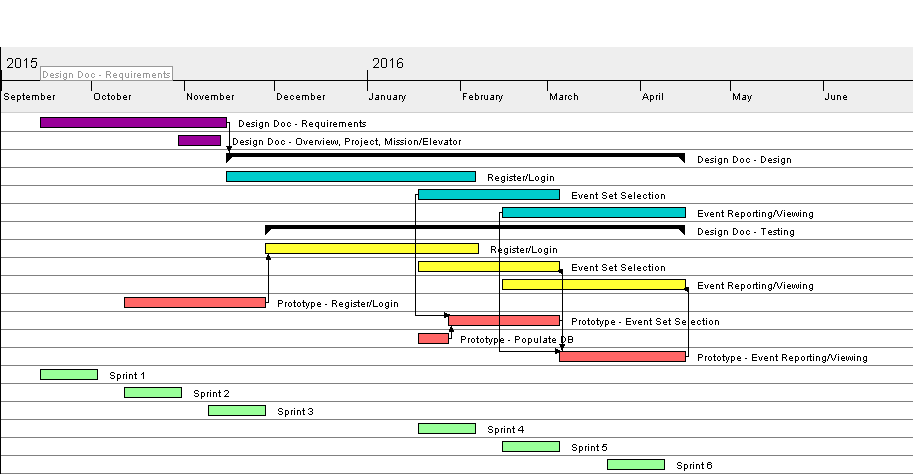
\includegraphics[width=0.75\textwidth]{./figures/projectgantt.png}
\end{center}
\caption{Gantt Chart of Project Completion Schedule\label{projectgantt}}
\end{figure}

\section{Backlogs}

\subsection{Sprint 1 Backlog}
\begin{itemize}
\itemsep0em
\item Documentation: start requirements section.
\item Review code from Landscape Change Mapper project.
\end{itemize}

\subsection{Sprint 2 Backlog}
\begin{itemize}
\itemsep0em
\item Documentation: requirements section, start project, overview and mission/elevator sections.
\item Implement Login/Register interface.
\item Prepare for first client presentation
\end{itemize}

\subsection{Sprint 3 Backlog}
\begin{itemize}
\itemsep0em
\item Documentation: project, overview and mission/elevator sections, start design and testing section for login/register.
\item Finish and test Login/Register interface.
\item Polish design document for first semester review.
\end{itemize}

\subsection{Sprint 4 Backlog}
\begin{itemize}
\itemsep0em
\item Documentation: prototype sections, revise requirements, design and testing section for login/register, start design section for set selection/list, and revised sprint plan in overview.
\item Add sample event reports and sample event set data to database. There will be a collection for each event set, one for information about the event set, and one for user login information.
\item Implement a select box to choose a different event set, and verify that the connection to the database is working as expected. The event report list will be started to verify accuracy of database.
\end{itemize}

\subsection{Sprint 5 Backlog}
\begin{itemize}
\itemsep0em
\item Documentation: design and testing section for set selection/list, start design section for report and map.
\item Implement reporting interface.
\item Finish implementing event report list.
\item Implement map interface.
\end{itemize}

\subsection{Sprint 6 Backlog}
\begin{itemize}
\itemsep0em
\item Finish Documentation: design and testing for report and map features, finalize sprint prototype and sprint report sections.
\item Final testing and debugging.
\item Polish prototype.
\item Design Fair preparation.
\end{itemize}


\section{Development Environment}
This section has information required to setup a development environment to run, test, and/or develop. 

\subsection{Development IDE and Tools}
No development IDEs were used. Code editing was done in a plaintext editor, Notepad++. More information about Notepad++ can be found at \url{https://notepad-plus-plus.org/}.

\subsection{Source  Control}
Source control is Github; github issues will be used to keep track of backlog and sprint status. The github repository is located at: \url{https://github.com/SDSMT-CSC464-F15/crowdscience} All parties have access to the Sprint and Product Backlogs.

\subsection{Dependencies}
The server requires Apache 2.2 and Mongo DB version 2.4.9 installed to run the project.

\subsection{Build  Environment}
The code in this project does not need to be built. The project uses scripted languages, which do not need compilation or building. 

\subsection{Development Machine Setup}
A remote desktop connection is required to connect to the server hosting the code. The rdp file for this remote desktop connection is show in Algorithm~\ref{alg_rdp}. The development machine should also install a plaintext editor such as Notepad++ to view and edit project files. 
\begin{algorithm} [tbh]                     
\caption{Remote Desktop Connection (.rdp) file}
\label{alg_rdp}    
\begin{lstlisting}
auto connect:i:1
full address:s: <IP address ommited>
username:s: <username ommited>
password:s: <password ommited>
\end{lstlisting}
\end{algorithm}


   %% All tracks
% !TEX root = SystemTemplate.tex
\chapter{User Stories, Backlog and Requirements}
\section{Overview}

This document contains project details for the Crowd Science Mapper project. The Crowd Science Mapper will be a generic crowdsourcing system framework and toolkits, which can be customized by ordinary users with no programming experience using graphical user interface

\subsection{Scope}

This section contain stakeholder information, initial user stories, requirements, and proof of concept results

\subsection{Purpose of the System}
The purpose of this system is to provide a generic crowdsourcing toolkit. That is, to allow ordinary to report and view events, and allow administrators to approve and modify event sets.

\section{ Stakeholder Information}

Stakeholders for this project are academics and researchers who would eventually be the users of this project.

\subsection{Customer or End User (Product Owner)}

Product owners are Dr. Mengyu Qiao and Gail Schmidt, who will assist in the project in mentor roles. As needed, they will assist with prioritizing the product backlog, and identify important features.

\subsection{Developers --Testers}
Developers and testers are Jiasong Yan and Hannah Aker.

\section{Requirements and Design Constraints}

This project will be a HTML based webpage using Java Script to connect to a Mongo database, and hosted on an Apache server

\subsection{System  Requirements}
Webpage should be able to run on all operating systems. This project is not required to have mobile functionality.


\subsection{Network Requirements}
This project will be server based, hosted on an Apache 2.0 server, access supplied to us by Gail Schmidt. 

\subsection{Development Environment Requirements}
Development will be done in HTML, PhP and Java Script. The project will connect to a Mongo database.

\subsection{Project  Management Methodology}
\begin{itemize}
\item Github issues will be used to keep track of backlog and sprint status.
\item All parties have access to the Sprint and Product Backlogs.
\item There will be 6 sprints total in this project.
\item Sprint cycles will last 3 weeks.
\item Source control will be Github.
\end{itemize}

\section{User Stories}

\subsection{User Story \#1}
As a user, I want all the core functionality of the landscape change mapper to be maintained. These functions include, but are not limited to:
\begin{itemize}
\item Visual map representation of events
\item Detailed event list
\item Event reporting interface
\item New user registration
\item User login
\end{itemize}

\subsection{User Story \#2} 
As an administrator, I want to be able to customize a set of events to fit my needs. This may include user input and display items, database design, digital map, webpage color and style, logo, etc. 

\subsection{User Story \#3} 
As an administrator, I want to be able to edit existing event reports.

\subsection{User Story \#4} 
As a user, I want to be able to select which set of events I would like to view.

\section{Supporting Material}
Project Description Document

  %% Not research track

% !TEX root = DesignDocument.tex

\chapter{Design  and Implementation}
This section contains the architecture and implementation details for each of the major components in the system.

 \section{Architecture and System Design}
 
 \subsection{Data Flow} 
 In general data flows from the HTML form to the associated JavaScript, which posts requests to PHP files to access data in the Database. See Figure~\ref{design_dataflow}.

\begin{figure}[tbh]
\begin{center}
\includegraphics[width=0.75\textwidth]{./figures/design_dataflow.png}
\end{center}
\caption{System Architecture and Design Overview\label{design_dataflow}}
\end{figure}
 
 \subsection{Communications} Data is communicated to and from the user via HTML. Data is communicated to and from the database via PHP and JavaScript to the HTML that the user sees. See Figure~\ref{design_dataflow}.
 
 \subsection{Databse Design} The database has a very flexible design, being a non-relational database. The database loosely resembles a relational database design, and differ in that a non-relational database can have a variable number of fields, and all fields are accessed via field name. There will also be a variable number of tables in the database. Four tables will remain constant: the User table, for storing user information; the Event Set Info, which stores information necessary for accessing tables containing the data for an event set; and the file storage tables, fs.files and fs.chunks, which are used to save uploaded files. Within the event set info table, the details section is an array containing information about how to access and display an event report. The remainder of the tables are variable, and store event reports for a given set. See Figure~\ref{design_database}.
 
  \begin{figure}[tbh]
\begin{center}
\includegraphics[width=0.75\textwidth]{./figures/design_database.png}
\end{center}
\caption{Database Design \label{design_database}}
\end{figure}
 
 \subsection{MVC} The project has a Model View Controller architecture. The model primarily consists of PHP files, which access the underlying data in the database. The view is the HTML files, which contain only page layout information. The controller is in the JavaScript, which controls dataflow to and from the view (HTML) and model (PHP) layer. See Figure~\ref{design_dataflow}.
 
 \subsection{GUI} See Figure~\ref{design_gui_index}, Figure~\ref{design_gui_login}, Figure~\ref{design_gui_register}, Figure~\ref{design_gui_report}, and Figure~\ref{design_gui_viewEvent}.
 
 \begin{figure}[!htbp]
\begin{center}
\includegraphics[width=0.75\textwidth]{./figures/design_gui_index.png}
\end{center}
\caption{GUI Design of Index Page \label{design_gui_index}}
\end{figure}

 \begin{figure}[!htbp]
\begin{center}
\includegraphics[width=0.75\textwidth]{./figures/design_gui_login.png}
\end{center}
\caption{GUI Design of Login Page \label{design_gui_login}}
\end{figure}

 \begin{figure}[!htbp]
\begin{center}
\includegraphics[width=0.75\textwidth]{./figures/design_gui_register.png}
\end{center}
\caption{GUI Design of Register Page \label{design_gui_register}}
\end{figure}

\begin{figure}[!htbp]
\begin{center}
\includegraphics[width=0.75\textwidth]{./figures/design_gui_viewEvent.png}
\end{center}
\caption{GUI Design of View Event Page \label{design_gui_viewEvent}}
\end{figure}

\begin{figure}[!htb]
\begin{center}
\includegraphics[width=0.75\textwidth]{./figures/design_gui_report.png}
\end{center}
\caption{GUI Design of Report Page \label{design_gui_report}}
\end{figure}
 
 \subsection{Technologies  Used}
Each major component uses the the major technologies: Apache server to access HTML documents, which use CSS and JavaScript, which posts to PHP to access the Mongo Database. See Table~\ref{technologies}.  

\section{Navigation Bar and User Selection of Event Set to Use}

\subsection{Component  Overview}
This component allows the user to navigate to other pages within the website. The navigation bar will contain links to register, login, logout, report an event, and return to the homepage. The login and register links will be replaced by the logout button when a user is logged in. The logout link will be hidden when no user is logged in. The link to the homepage will always be present. The report event link will be hidden on the login, register, and view individual event pages. The register link will be hidden on the register and view individual event pages. The login link will be hidden on the login and view individual event pages. The navigation bar will contain a dropdown selection box for selecting an event set to view and use. The selection box will be hidden on the register, login, and and view individual event pages. When the event set selection is changed, the fields on the report event page will change to reflect the current event set and the data on the main page will change to reflect the selected event page.

\subsection{Phase Overview}
This component was parially adapted from existing Landscape Change Mapper code. New features were added to the existing navigation bar in the LCM code: the event set selection box and the report link. This component was partially implemented in phase one, adapting LCM code, and in phase two, adding Crowd Science Mapper features.

\subsection{ Architecture and Dataflow Diagram}
See Figure~\ref{design_navbar}.
\begin{figure}[tbh]
\begin{center}
\includegraphics[width=0.75\textwidth]{./figures/design_navbar.png}
\end{center}
\caption{Dataflow and Architecture of Navigation Bar and Event Set Selection Component \label{design_navbar}}
\end{figure} 

\subsection{Design Details}
To maintain state as the user moves from page to page, the currently selected event set is stored in the PHP's session data. When the selection is changed, the JavaScript sends the new selection in a POST to event.php, where the current selection is saved to the session data and current event set options are retrieved from the database.  The data in the PHP file is then echoed back to the JavaScript that made the POST, and the JavaScript executes code to update the selection box in the HTML. See Figure~\ref{design_navbar} for the specific functions called to accompish this. 

\section{User Registration, Login, and Logout}

\subsection{Component  Overview}
This component allows the user to register, login, and logout. When the user clicks the register link inthe navigation bar, the user will be taken to the register page. The register page will contain at least feilds for username, password, and password verification, which will be required fields. When a user clicks submit, their input is checked. If the user has not filled out all required fields or their passwords do not match, the user will be notified. After the user has registered, they will be automatically logged in. When the user clicks the login link in the navigaton bar, they will be taken to the login page. The login page will contain username and password fields. When the login button is clicked, the user's input is checked. If the username or password is incorrect, the user is notified. When the user sucessfully logs in, they are redirected to the main page. When a user clicks the logout link on the navigation bar, the user will be logged out, and redirected to the main page.

\subsection{Phase Overview}
This component was almost entirely adapted from existing Landscape Change Mapper code, and thus, implemented primarily in phase one of the project, adapting LCM code. 

\subsection{ Architecture and Dataflow Diagram}
See Figure~\ref{design_login_register_logout}.
\begin{figure}[tbh]
\begin{center}
\includegraphics[width=0.75\textwidth]{./figures/design_login_register_logout.png}
\end{center}
\caption{Dataflow and Architecture of Login, Register, and Logout Component \label{design_login_register_logout}}
\end{figure}

\subsection{Design Details}
To keep the user logged in as the user moves from page to page, the user's username is stored in the PHP's session data. When a user logs out, the username field is cleared from session data. 

The login form contains a text field for the username, a password field for the user's password, a button to submit the form data, and a button to cancel and return to the home page. The login page also contains a link to the register page, in addition to the register link in the navigation bar.  To prevent multiple logins, the page checks to see if a user is already logged in, and if one is, redirects to the home page. When the user clicks the submit button, the data is sent to the PHP, which checks it against the database and returns errors if it doesn't match. Error messages will be shown to the user. If the data matches, then the username is updated in the session data, and the user is redirected to the index page. 

The register form contains text fields for the user's email, username, first name, last name, and location; passwords fields for the user's password and password verification; and a selection box for the type of user. When the user clicls the submit button, the Javascript checks that the passwords on the form match, and then sends the data to the PHP. The PHP first checks to see if the username or email have already been used in the database, and returns an error message if they have been used. Otherwise, the user's information is added to the database, and the user is logged in and redirected to the index page.

\section{Generic Event Reporting Interface}

\subsection{Component  Overview}
This component allows the user to report an event for the event set they have selected. The event reporting window will contain a map for selecting the location of the event, with the latitude and longitude displayed underneath. If the latitude and longitude text boses are changed, the map will reflect the change. The user will be able to fill out the fields specific to the event set they have selected. When the user changes the event set, the fields will also change. The user will have the option to upload multiple photos with their event report. When the user clicks submit, the event report will be added to the database.

\subsection{Phase Overview}
This component was primarily part of phase two, adding Crowd Science Mapper code. While this component used some existing Landscape Change Mapper code, the changing fields on the page required a lot of new code. The map for selecting the report location and the photo upload interface are adapted from LCM code.

\subsection{ Architecture and Dataflow Diagram}
See Figure~\ref{design_report}.
\begin{figure}[tbh]
\begin{center}
\includegraphics[width=0.75\textwidth]{./figures/design_report.png}
\end{center}
\caption{Dataflow and Architecture of Event Reporting Component \label{design_report}}
\end{figure} 

\subsection{Design Details}
When the report page is loaded or refreshed, the page checks to see if a user is currently logged in. If a user is logged in, the links shown on the navigation bar change accordingly. 

When the selected event is changed, the fields on the report page update accordingly. After the field information is retrieved from the database, the list of fields are looped through. For each field, a new object is generated within the Javascript, and stored so that the object may later be accessed to upload the user's report. A different type of object will be added, depending on the feild type. Field types include selection, number, date, short text, and long text. A list of selection options accompanies a selection field's info, and number range and step accompany a number field's info. The object ids directly match the field name for the object's storage in the database. The objects are stored because JQueries are made for accessing elements of an HTML file, and cannot access things added to the HTML file after it has been loaded. 

The map on the report page is created from custom LCM code that simplifies the map API so that a user may only select one location, and the location is tracked with latitude and longitude fields on the report form. When the latitude and longitude fields on the report form are changed, the location indicated on the map also changes. 

To upload photos, the user must select the photos from their device, and then click on the upload photos button. When the user clicks on this button, the photos are uploaded to the database, and checked to see if they contain location information. If the photos contain location information, the latitude and longitude on the report form are updated. The Mongo Ids of the uploaded files are then saved to be added to the report when it is submitted.

When the report is submitted, the saved field objects are looped through to extract the stored information. The id of each object corresponds to the field name it is stored as in the database, so the object id is used as the index into the array that the fields are stored in for posting to the PHP file. The photo IDs saved when the photos were uploaded are added as an array to the photos field in the PHP request array. Latitude and longitude are also added to the array, and the array is sent to the reprt PHP file. In the report PHP file, the photo IDs are all changed to Mongo IDs, the date is changed to the Mongo date format, and the latitude and longitude are combined into an array. If there is a username stored in session data, the report author is set to that user's ID. Otherwise, the report author is listed as annonymous.The report is then added to the database, and the user is returned to the index page. 

\section{Generic Event Set Viewing}

\subsection{Component  Overview}
This component allows the user to view event reports in a variatey of ways. The user can view the event set reports as pins on a map interface. When the user clicks on a pin, a brief summary of the report is shown to the user, and the user can click on the summary to go to the individual event's page. The user can view the event set in a table. Each row will contain information about an event report, including author, and event report details. The user can click on the links in each row to go to the individual event's page, or to zoom to the event on the map. The user can view the images in an event set via the image carousel. The image carousel will periodically display a different event report's image, and the user can mannually nagivate the images with the arrows on either side of the carousel. The user can also view an individual event's page. The individual event's page will have all of the images for the event report, the exact latitude and longitude of the report, the author, and the other details associated with the report.

\subsection{Phase Overview}
The majority of this component was implemented in phase two, adding Crowd Science Mapper code. The event map, table, and individual event page from the Landscape Change Mapper all had to be largely rewritten to accomidate a variable set of details. The image carousel was more easily adapted from LCM code.

\subsection{ Architecture and Dataflow Diagram}
See Figure~\ref{design_viewing}.
\begin{figure}[tbh]
\begin{center}
\includegraphics[width=0.75\textwidth]{./figures/design_viewing.png}
\end{center}
\caption{Dataflow and Architecture of Event Viewing Component \label{design_viewing}}
\end{figure} 

\subsection{Design Details}
When the event set selection is changed, or the index page is refreshed, the event set table, map, and image carousel should be updated with new data from the database.

When the new information from the database is retrieved, the event set table first replaces its headers with the event set information contained in the database.

These sections should connect the backlog items listed to the refman sections - map how I got from the requirement to the actual code.

  %% All tracks
% !TEX root = DesignDocument.tex


\chapter{System  and Unit Testing}

\section{Overview}
This section describes the approach taken with regard to system and unit testing. Testing is done manually, via a traceability matrix. Each requirement listed in the backlog will have a test case and list the code that is covered by the test case.  

\section{Test Set-up and Execution}
Each major component has a list of requirements. Test cases are generated to ensure that each requirement has been thoroughly tested, to ensure that the requirement has been fulfilled. Each test case will also list the functions and files that the test case specifically tests. Requirements that are present in the test case but the test case isn't directly testing, will not be listed as a requirement fulfilled by that test case. The code coverage refers to the file documentation section of this document.

Automated testing was not implemented in this project, but manual testing was performed along the course of the project to ensure product functionality. The test cases for this manual testing are listed below.

\section{System Testing}

\subsection{Navigation Bar Test Cases}
\begin{itemize}
\item Navigate to all website pages and confirm presence of navigation bar.
\item Confirm home, report, and logout buttons, and user logged in icon, in the navigation bar on the index page when a user is logged in
\item Confirm home, report, register, and login buttons in the navigation bar on the index page when a user is not logged in 
\item Confirm home and logout buttons, and user logged in icon, in the navigation bar on the report page when a user is logged in
\item Confirm home, register and login buttons in the navigation bar on the report page when a user is not logged in
\item Confirm home, report, and register buttons in the navigation bar on the login page
\item Confirm home, report, and login buttons in the navigation bar on the register page
\item Confirm home and report buttons in the navigation bar on the view event page
\item Confirm event set selection box on index and report pages
 \end{itemize}
\subsubsection{Result}
Passed test cases:
\begin{itemize}
\item When no user is logged in, there are a home button, an event set selection box, a report button, a login button, and a register button in the navigation bar on the home page.
\item When no user is logged in, there are a home button, an event set selection box, a login button and a register button in the navigation bar on the report page.
\item There are home, report, and login buttons in the navigation bar on the register page.
\item There are home, login, and login buttons in the navigation bar on the login page.
\item There are home and report buttons in the navigation bar on the view event page.
\item When a user is logged in, there are a home button, an event set selection box, a report button, a user icon, and a logout button in the navigation bar on the home page.
\item When a user is logged in, there are a home button, an event set selection box, a user icon, and a logout button in the navigation bar on the report page.
 \end{itemize}
\subsubsection{Code Coverage}
\begin{itemize}
\item checkLogin.js: document ready ( )
\item checkLogin.js: POST\_CheckLogin ( )
\item checkLogin.php
\item checkLogin.js: UpdateUserStatus ( )
\item login.php
\item config.php
\item index.html
\item login.html
\item register.html
\item report.html
\item viewEvent.html
\end{itemize}
\subsubsection{Requirements Fulfilled}
\begin{itemize}
\item Each page shall contain a navigation bar at the top of the page.
\item The navigation bar will have buttons for logging in, new user registration, logout, and event reporting, where appropriate.
\item When no user is logged in, there will be buttons in the navigation bar leading to a new user registration page and a user login page.
\item When the user is logged in, an icon indicating the logged in user and a log out button will replace the login button on the navigation bar.
\end{itemize}

\subsection{Event Set Selection Test Cases }
\begin{itemize}
\item Change data stored in database, verify that selection boxes update with database data when page is refreshed. 
\item Select event set on index page, navigate to report page, verify that selection was maintained. Refresh page and verify that selection was maintained. 
\item Change event set selection, verify that data on index page and report fields update with appropriate data.
\item Verify error message when event set options cannot be updated due to no database connection. 
\end{itemize}
\subsubsection{Result}
Passed test cases:
\begin{itemize}
\item Added Pine Beetle Spread event set to database, refreshed page. Pine Beetle Spread appeared in selection box. Removed Pine Beetle Spread from data base, selected different set. Pine Beetle Spread no longer appeared in selection box. 
\item Selected Bird Sightings on index page, navigated to report page. Event set selection maintained Bird Sightings as selected event set. Refreshed the page. Event set selection maintained Bird Sightings as selected event set. 
\item Changed selection on report page from Bird Sightings to Pine Beetle Spread. Report fields updated: date, description, number of birds, and species updated to date, additional details, number of infected trees, and tree species targeted. 
\item Changed selection on home page from Pine Beetle Spread to Wildflower Sightings. Page updated from empty page to show Wildflower Sightings event set data.
\item Removed database connection in config.php, refreshed index. Page alerted ``500: Error loading Event Set Options''.
\end{itemize}
\subsubsection{Code Coverage}
\begin{itemize}
\item event.php: changeEventSetSelection ( )
\item event.php: updateEventSetOptions ( )
\item index.js: POST\_ChangeEventSetSelection ( )
\item index.js: POST\_UpdateEventSetOptions ( )
\item index.js: UpdateEventSetOptions ( )
\item report.js: POST\_ChangeEventSetSelection ( )
\item report.js: POST\_UpdateEventSetOptions ( )
\item report.js: UpdateEventSetOptions ( )
\end{itemize}
\subsubsection{Requirements Fulfilled}
\begin{itemize}
\item The navigation bar shall contain a drop down box for selecting the event set.
\item The selected event set shall maintain its state when navigating to a different page or refreshing the page.
\item When the current event data set is changed, the map, event list, image carousel, and report features will change according to the feilds specified for that set.
\end{itemize}

\subsection{ New User Registration Test Cases}
\begin{itemize}
\item Confirm register page contains fields for user to enter username, password, and password verification, and a submit button.
\item Confirm that cancel button takes user to index page.
\item When user does not fill all required fields, verify error message.
\item When user submits registration with mismatched passwords, verify error message.
\item Verify error message for email or username already taken.
\item When user successfully submits report, verify data in database.
\item Verify user is logged in after registering.
\item Login, and navigate to the register page via the address bar, register a new user, verify old user is logged out, and new user logged in.
\end{itemize}

\subsubsection{Result}
Passed test cases:
\begin{itemize}
\item There are fields for email, username, password, password verification, first name, last name, user role, and location, and buttons to create account and cancel on register page.
\item Clicking cancel button redirects user to index page.
\item When the user clicks submit without filling out any fields, box appears with ``please fill out this field''.
\item When the user enters mismatched passwords and clicks submit, box appears with ``Passwords Don't Match'' and password fields are cleared.
\item When the user enters a username that has already been taken, box appears with ``Username already taken''.
\item When the user enters an email that has already been taken, box appears with ``Email Already Registered''.
\item When the user enters mismatched passwords, fixes it and enters an email that is already taken, verify that password error message disappears and email taken error message appears, and vice versa.
\item When the user enters mismatched passwords, fixes it and enters a username that is already taken, verify that password error message disappears and username taken error message appears, and vice versa.
\item When the user enters a username that has been taken, fixes it and enters an email that is already taken, verify that user taken error message disappears and email taken error message appears, and vice versa.
\item When the user enters text in the email box that does not match the standard email form, box appears and informs user that email does not contain the @ sign.
\item When the user correctly enters email address, username ``haker3'', and passwords and clicks submit, entry appears in database, user redirected to index page, and index navigation bar changes to show ``haker3'' logged in.
\item Logged in as ``haker2'', navigated to register page via address bar, registered new user ``haker4'', logged in as ``haker4'' and redirected to index page.
\end{itemize}
\subsubsection{Code Coverage}
\begin{itemize}
\item register.html
\item register.js: document ready ( )
\item register.js: POST\_RegisterUser ( )
\item register.js: OnRegisterSuccess ( )
\item register.php 
\item register.php: registerUser( )
\end{itemize}
\subsubsection{Requirements Fulfilled}
\begin{itemize}
\item The registration page will have a field for username, password and password verification, and a ``submit'' button.
\item If the passwords do not match, the user will be notified, and need to re-enter one or both passwords.
\item After registering, a user will automatically be logged in.
\end{itemize}

\subsection{User Login Test Cases}
\begin{itemize}
\item Confirm login page contains fields for user to enter username or email and password, a submit button, and a link to the user registration page.
\item When user enters a user name or email not in the database and clicks submit, verify error message.
\item When user enters password that does not match database and clicks submit, verify error message.
\item When user enters correct email and password and clicks submit, verify user is logged in.
\item When user enters correct username and password and clicks submit, verify user is logged in.
\item Confirm that cancel button takes user to index page.
\item Login, and navigate to the login page via the address bar, verify user is redirected to index.
\end{itemize}
\subsubsection{Result}
Passed test cases:
\begin{itemize}
\item Login page contains username/email and password fields, submit button, cancel button, and link to register page.
\item When user enters incorrect username, email, or password, the error message ``The username and password combination could not be found'' is displayed.
\item When user enters correct email and password and clicks submit, the user is logged in and taken to index page.
\item When user enters correct username and password and clicks submit, the user is logged in and taken to index page.
\item Clicking cancel button redirects user to index page.
\item Logged in as ``haker3'' and navigated to login page, redirected to index page.
\end{itemize}
\subsubsection{Code Coverage}
\begin{itemize}
\item login.js: POST\_CheckLoginStatus ( )
\item login.js: POST\_LoginUser ( )
\item login.js: OnLoginSuccess ( )
\item login.js: document ready ( )
\item login.php: validateUser ( )
\item login.php
\end{itemize}
\subsubsection{Requirements Fulfilled}
\begin{itemize}
\item The login page will have fields for entering username and passwords, a ``login'' button and a link to the user registration page.
\item The user will be notified if the username or password was incorrect, and may need to re-enter one or both fields.
\end{itemize}

\subsection{Event Reporting Interface Test Cases}
\begin{itemize}
\item Confirm report page contains map for selecting latitude and longitude, event set fields, image upload interface, and submit button.
\item Click on map, verify latitude and longitude change.
\item Change latitude and longitude, verify map marker changes.
\item Verify map zoom in and out.
\item Verify report fields match database fields. Verify selection box options match database. Verify step, max and min for number match database.
\item Verify image upload of one image. Verify image upload of two images.
\item Verify report submission for report with no image, one image, and two or more images. 
\item Verify report's author is ``anonymous'' when a user isn't logged in and submits a report.
\item Verify report's author matches logged in user when a logged in user submits an event report.
\item Verify submitted event report contains latitude and longitude.
\item Verify database report matches submitted report.
\end{itemize}
\subsubsection{Result}
Passed test cases:
\begin{itemize}
\item There are a map for selecting latitude and longitude, event set fields, image uploading interface, and submit button on the report page, when the Wildflower Sightings event set is selected.
\item Clicked on map, latitude and longitude updated to match location.
\item Changed latitude, map updated to match new latitude. Changed longitude, map updated to match new longitude.
\item Event report fields: date, description, number of flowers, and species; match fields and types in database. Number of flowers step value is 1 and does not decrement below zero, matching min and step value in database. Landscape Changes' category selection box options match selection options in database. 
\item Submitted anonymous report with no pictures to ``Pine Beetle Spread''. Report in database matches information entered.
\item Submitted anonymous report with one picture to ``Pine Beetle Spread''. Report and picture in database matches information entered and photo uploaded.
\item Submitted anonymous report with two pictures to ``Pine Beetle Spread''. Report and pictures in database matches information entered and photos uploaded.
\item Submitted report with two pictures to ``Pine Beetle Spread''. Report and pictures in database matches information entered and photos uploaded. Report author saved in database matched user submitting report.
\end{itemize}
Failed test cases:
\begin{itemize}
\item Changed latitude and longitude to the south pole (-90,180) for fun, and clicked back in South Dakota. The longitude for Rapid City was approximately 256, where it is supposed to be approximately -103. The western half the the hemisphere is unaffected by this glitch. However, when the longitude is changed to -180, the error repeats respectively with the western half of the hemisphere. Clicking over the line international date line, at longitude -180 or 180, in one direction or the other will cause this error. This is a known bug in the map API used, outside the scope of the project. 
\end{itemize}
\subsubsection{Code Coverage}
\begin{itemize}
\item event.php: getEventSetData ( )
\item fileUpload.php
\item report.js: POST\_SubmitEventReport ( )
\item report.js: POST\_UpdateReportFields ( )
\item report.js: POST\_UploadPhotos ( )
\item report.js: document ready ( )
\item report.js: UpdateReportFields ( )
\item report.php: submitEventReport ( )
\item report.php
\item reportMapLeaflet.js: initmap ( )
\item reportMapLeaflet.js: addMarker ( )
\item reportMapLeaflet.js: onMapClick ( )
\item reportMapLeaflet.js: onChangeLatLong ( )
\end{itemize}
\subsubsection{Requirements Fulfilled}
\begin{itemize}
\item The event reporting window shall contain a map for selecting the latitude and longitude of the event.
\item The event reporting window shall contain the fields specified for that event data set.
\item The event reporting window shall contain an interface for uploading images with the event report.
\item The event reporting window shall contain a submit button.
\item When the user clicks submit, the report is added to the database.
\item When a user is logged in, the user is listed as the author of the report.
\item When no user is logged in, the author of the report is saved as ``Anonymous''.
\item Every event report shall include a longitude and latitude field.
\end{itemize}

\subsection{Detailed Event List Test Cases}
\begin{itemize}
\item Verify that event set table header contains User and all event set details fields. Verify that table body contains user and all  event set details fields.
\item Verify that clicking on zoom icon zooms map to the event in the associated table row. 
\item Verify that clicking the link icon in the event table takes user to individual event page.
\end{itemize}
\subsubsection{Result}
Passed test cases:
\begin{itemize}
\item Selected Pine Beetle Spread. The event set table headers contain User, Date, Additional Details, Number of Infected Trees, and Tree Species Targeted. Table body contained information in the correct column of user and all event report details. 
\item Clicked on zoom icon in first row of table, map zoomed to the event in that row, the map pop-up information matched the event.
\item Clicked on link icon in the second row of the table, the information in the individual event page matched the row containing the link.
\end{itemize}
\subsubsection{Code Coverage}
\begin{itemize}
\item event.php: getEventSetInfoAndData ( )
\item index.js: POST\_UpdateEventSetTableAndMap ( )
\item index.js: document ready ( )
\item index.js: UpdateEventSetTable ( )
\end{itemize}
\subsubsection{Requirements Fulfilled}
\begin{itemize}
\item The detailed event list will be a table of the current event set, and will include all fields specified for that event data set.
\item Each entry shall include the author of the event.
\item Each entry shall include links to the individual event page and to center the map on that event.
\end{itemize}

\subsection{Map Representation of Events Test Cases}
\begin{itemize}
\item Confirm that the map contains a marker for each event in the event set. Verify each event marker is at the correct latitude and longitude for the report.
\item Confirm that a pop-up with event details appears when a marker on the map is clicked. 
\item Confirm that when a pop-up on the map is clicked on, it takes the user to the individual event page for that event.
\item Verify that map can be panned and zoomed in and out.
\end{itemize}
\subsubsection{Result}
Passed test cases:
\begin{itemize}
\item All event markers were present on the map, and each was in the location reported by the user, including the event with an incorrect longitude of -214, per the map API bug found in the report testing.
\item Clicked on a marker for an event with no photos, event details popped up and displayed all event details for the specific event. Clicked on a marker for an event with photos, event pop-up displayed photo and all details. 
\item Clicked on event pop-up, automatically navigated to individual event page for that event report. All information matched.
\item Click and dragged to pan map, map panned. Used arrow keys to pan map, map panned. Used scroll to zoom in and out, map zoomed in and out. Used map buttons to zoom in and out, map zoomed in and out.
\end{itemize}
\subsubsection{Code Coverage}
\begin{itemize}
\item event.php: getEventSetInfoAndData ( )
\item image.php
\item index.js: POST\_UpdateEventSetTableAndMap ( )
\item index.js: document ready ( )
\item index.js: UpdateEventSetMap ( )
\end{itemize}
\subsubsection{Requirements Fulfilled}
\begin{itemize}
\item The map shall contain a marker for each event report, placed at the longitude and latitude specified in the report.
\item When a marker on the map is clicked on, a pop-up will appear with the picture associated with the event report, and the event report details. 
\item When an event report pop-up is clicked, the user will be navigated to the individual event page.
\item The map will be able to be zoomed in, zoomed out, and panned.
\end{itemize}

\subsection{Event Set Image Carousel Test Cases}
\begin{itemize}
\item Verify that the image carousel contains one image per event in the event set.
\item Verify that the image carousel periodically displays a new image.
\item Verify user can navigate pictures with image carousel arrows.
\end{itemize}
\subsubsection{Result}
Passed test cases:
\begin{itemize}
\item For the Pine Beetle Spread event set, there are 3 images in the image carousel, and 3 events in the event set that contain images. 
\item The image carousel moves to the next image in the set every few seconds.
\item Clicked on the right arrow in the image carousel, was taken to the next photo in the event set. Clicked on the left arrow in the image carousel, was taken to the previous photo in the event set.
\end{itemize}
\subsubsection{Code Coverage}
\begin{itemize}
\item event.php: getEventSetInfoAndData ( )
\item image.php
\item index.js: POST\_UpdateEventSetTableAndMap ( )
\item index.js: document ready ( )
\item index.js: UpdateEventSetImageCarousel ( )
\end{itemize}
\subsubsection{Requirements Fulfilled}
\begin{itemize}
\item The image carousel will contain one image per event in the selected event set.
\item The image carousel will periodically display a different event image.
\item The user will be able to navigate through the pictures in the image carousel using arrows at the sides of the image carousel.
\end{itemize}

\subsection{Individual Event Viewing Test Cases}
\begin{itemize}
\item Verify that individual event page contains information matching the event that was clicked on in the previous page. 
\item Verify that individual event page contains image carousel with all pictures associated with the event. 
\item Verify the individual event page contains the reporting user, latitude and longitude of the event.
\item Verify that the individual event page contains all details about the event.
\end{itemize}
\subsubsection{Result}
Passed test cases:
\begin{itemize}
\item Clicked on a pop-up in the map, individual event page matched map pop-up. Clicked on table link, individual event page matched table row. 
\item Individual event page contains all photos for event, clicked on event with two photos, both photos present in individual event image carousel.
\item Individual event page contained user, latitude, longitude, and all details matching event in database.
\end{itemize}
\subsubsection{Code Coverage}
\begin{itemize}
\item event.php: getEventSetInfoAndEventByID ( )
\item image.php
\item viewEvent.js: DisplayEvent ( )
\item viewEvent.js: POST\_GetEventSetInfoAndEventByID ( )
\item viewEvent.js: document ready ( )
\end{itemize}
\subsubsection{Requirements Fulfilled}
\begin{itemize}
\item The individual event page will contain only information regarding the event clicked on by the user on a previous page.
\item The individual event page will contain all pictures associated with an event.
\item The individual event page will contain the specific latitude and longitude associated with an event.
\item The individual event page will contain all details pertaining to the event.
\end{itemize}

\section{System Integration Analysis}
The system is a designed as a website, and would need to be integrated in to the world wide web. This integration would involve registering a domain name for the system, and dedicating a server to running the system for public use. Other mapping systems, such as the USGS Did you Feel it (DYFI) project and the USGS Butterflies and Moths of North America (BAMONA), may need to be integrated with this system later. Integration with these other systems will need to be done by hand.

\section{Risk Analysis}
Risks of this project include server capabilities, server crash, database crash, database hacking, and map API bugs.

The server currently has good load handling capabilities, but lacks storage space for a large number of event reports. The Apache 2.2 server has good load capabilities. When testing 90 concurrent users each doing 30 page hits, the mean number of requests per second was 5244.86, and 95\% of requests were handled within 16 ms. The server itself has 6.92 GB of free space. The Crowd Science Mapper database currently uses 201326592 bytes, or about .2 GB. The database currently contains a total of 23 event reports. Thus, one event report requires roughly 0.009 GB of space. The system currently has enough space to store 650-750 event reports total. The database has a large pool of connections that can be used. There are currently 21 connections in use, and 19979 connections available. 

The server and database are both very stable, with good up times. The chances of a server or database crash are small, with the good load handling capabilities of both. The server is regularly maintained, and in good condition. Currently, all project files are backed up on GitHub, and all the scripts and files used to create the project database are also backed up on GitHub. In the event of loosing all data, the current project could be recreated relatively easily.

Database security is an issue. The users' passwords are stored as plain text in the database.  Though NoSQL database, such as the Mongo Database used in this project, are less vulnerable to injection attacks, user input is not fully sanitized before being sent as a database query. Currently, a malicious user would be unable to change any database information, all database interaction is performed through insert and find operations. An experienced malicious user could potentially view user data, including user passwords through an injection attack. 

There is a bug with the map API used - the map's longitude does not properly wrap around the international date line. This may cause reports to have incorrect longitude, however, reports with incorrect longitude like this still behave correctly on the map.

\subsection{Risk Mitigation}
To scale up the project, the first thing that would need to happen is expansion of available database memory. Past that, to handle heavy traffic, caches should be utilized to increase user speed, such as PHP OpCode caching, client-side web-page caching of static web-pages, database caching of common queries, and database load balancing. 

The server should be periodically backed up when the project is past the development and testing stages, and being used for real crowd science projects. Depending on how often event reports are submitted, the server should be backed up weekly, for very light usage, to daily, for heavy usage. 

Before entering beta testing of any sort, passwords need to be encrypted when stored in the database. This is listed as a feature in the future work section of this document. User input also needs to be sanitized for database queries. 

The map API doesn't cause any fatal errors, and can be left as is. However, future project work should include looking into other map APIs for use with the project.

  %% All tracks
% !TEX root = SystemTemplate.tex
\chapter{Development Environment}


 %% All tracks
%%% !TEX encoding = UTF-8 Unicode
% !TEX root = DesignDocument.tex

\chapter{Release -- Setup -- Deployment}
This section should contain any specific subsection regarding specifics in releasing, 
setup, and/or deployment of the system. 


\section{Deployment Information and Dependencies}
Are there dependencies that are not embedded into the system install? 



\section{Setup Information}
How is a setup/install built? 



\section{System  Versioning Information}
How is the system versioned? 
  %% Normally not research track
% !TEX root = DesignDocument.tex

\chapter{User Documentation}
End user documentation covers basic steps for using the crowd science mapper, and basic commands for editing and uploading information to the Mongo Database.

\section{User Guide}
\begin{itemize}
\item To view an event set, go to the index page, and select an event set with the selection box in the navigation bar. 
\item To view information about a marker on the map, simply click the marker. 
\item To view more information about an event, click the pop-up on the map for the event, or the link icon in the table below. 
\item To center the map on an event, click the zoom icon in the table below. 
\item To navigate the image carousel, use the arrow at either side of the image carousel. 
\item To report an event, click the report button, and fill out the form. When submitting images, select a file using the select file button, and then upload your images before submitting the report with the upload button. To select the location of the report, click anywhere on the map. 
\item To login, click the login link, and fill in your email or username and password, and click login. 
\item To register, click the register link, fill out the required fields in the form, and click register.
\end{itemize}
\section{Database Administration Guide}
This is a quick reference guide to the commands used in this project to interact with the Mongo Database. On the server, the Mongo DB application is located at ``C:/mongodb/bin/mongo.exe''. Clicking on the executable will open the Mongo shell. The Mongo shell can also be accessed via command line. 

To list the databases available, use the command ``show dbs'', see Figure ~\ref{show_dbs}.
\begin{figure} [tbh]                     
\caption{Mongo Database: List Databases}
\label{show_dbs}    
\begin{lstlisting}
> show dbs
comedy  0.203125GB
crowdsciencemapper      0.203125GB
lcmapper        0.453125GB
local   0.078125GB
\end{lstlisting}
\end{figure}
To select a different database, use the command ``use <database>'', see Figure~\ref{use_db}.
\begin{figure} [tbh]                     
\caption{Mongo Database: Select Database}
\label{use_db}    
\begin{lstlisting}
> use crowdsciencemapper
switched to db crowdsciencemapper
\end{lstlisting}
\end{figure}
To load JavaScript code, use the command ``load(``<filename>'')'', see Figure~\ref{db_load_file}. For sample JavaScript code to add users to the database manually, see Figure~\ref{db_init_users}.   For sample JavaScript code to add new event sets to the database, see Figure~\ref{db_init_eventsetsinfo}.
\begin{figure} [tbh]                     
\caption{Mongo Database: Load File}
\label{db_load_file}    
\begin{lstlisting}
> load("db\_user\_init.js")
true
\end{lstlisting}
\end{figure}

\begin{figure} [tbh]                     
\caption{Mongo Database: db\_user\_init.js}
\label{db_init_users}    
\begin{lstlisting}
db.user.drop();

db.user.insert({ 
_id : ObjectId("546e81372f32a09417000048"), username : "danhalloran", 
email : "drhalloran@gmail.com" , password : "asdf", score : "0", 
details : {  lname : "Halloran" , fname : "Dan", 
location : "Rapid City, SD, USA" , role : "Citizen"} 
});

db.user.insert({ 
_id : ObjectId("5629c3362f32a0940e000029"), username : "haker", 
email : "hannah.aker@mines.sdsmt.edu" , password : "password",  score : "0", 
details : { lname : "Aker",  fname : "Hannah", 
location : "Okalhoma City, OK, USA" , role : "Citizen"} 
});

\end{lstlisting}
\end{figure}

\begin{figure} [tbh]                     
\caption{Mongo Database: db\_eventsetsinfo\_init.js}
\label{db_init_eventsetsinfo}    
\begin{lstlisting}
db.eventsetsinfo.drop();

db.eventsetsinfo.insert({ 
id : "wildflower", name : "Wildflower Sightings",
details : [ 	{ id : "species", name : "Species", type : "shorttext"},
		{ id : "count", name : "Number of Flowers", 
			type : "number", min : "0", max : "none", step : "1"},
		{ id : "description", name : "Description", type : "longtext"},
		{ id : "date", name : "Date", type : "date" } ]
			});
			
db.eventsetsinfo.insert({ 
id : "landscapechange", name : "Landscape Changes",
details : [ 	{ id : "nat_event_name", name : "Natural Event Name", 
		type : "shorttext"},
		{ id : "category", name : "Category", type : "selection", 
			options : [	{id :"fire", name : "Fire"},
					{id :"wind", name : "Wind Damage"},
					{id :"avalanche", name : "Avalanche Damage"},
					{id :"timber", name : "Thinning/Timber Harvest"},
					{id :"insect", name : "Insect Infestation"},
					{id :"landslide", name : "Landslide"},
					{id :"earthquake", name : "Earthquake"},
					{id :"flooding", name : "Flooding"},
					{id :"mining", name : "Surface Mining"},
					{id :"construction", name : "Road/House Construction"}]		   
			},
		{ id : "status", name : "Status", type : "selection", 
			options : [	{id : "ongoing", name : "Ongoing"},
					{id : "finished", name : "Finished"}]
			},
		{ id : "size", name : "Size", type : "selection", 
			options : [	{id : "large", name : "Larger than Baseball Diamond"},
					{id : "small", name : "Smaller than Baseball Diamond"}]
			},
		{ id : "description", name : "Description", type : "longtext"},
		{ id : "date", name : "Date", type : "date"} ]
			});
\end{lstlisting}
\end{figure}

To load an image to the database, use the ``mongofiles'' command directly from the command line, see Figure~\ref{db_load_image}. To insert an event set with and image already uploaded use the Mongo ID of the image in loading a JavaScript insert operation, see Figure~\ref{db_init_wildflower}.

\begin{figure} [tbh]                     
\caption{Mongo Database: Load File}
\label{db_load_image}    
\begin{lstlisting}
C:\mongodb\bin>mongofiles -d crowdsciencemapper put dbscripts\Pasque1.jpg
connected to: 127.0.0.1
added file: { _id: ObjectId('56d3af7e68b32cd77194a193'), filename: "dbscripts\Pa
sque1.jpg", chunkSize: 262144, uploadDate: new Date(1456713598460), md5: "c04035
a5d84940a6f75b17e5eece7433", length: 19061 }
done!

C:\mongodb\bin>mongofiles -d crowdsciencemapper put dbscripts\Pasque2.jpg
connected to: 127.0.0.1
added file: { _id: ObjectId('56d3af8322f00a38e3989dd7'), filename: "dbscripts\Pa
sque2.jpg", chunkSize: 262144, uploadDate: new Date(1456713603078), md5: "436817
a4c6eaf70ba8a0f23f71297549", length: 168395 }
done!
\end{lstlisting}
\end{figure}

\begin{figure} [tbh]                     
\caption{Mongo Database: db\_wildflower\_init.js}
\label{db_init_wildflower}    
\begin{lstlisting}
db.wildflower.insert({ 
user : ObjectId("5629c3362f32a0940e000029"), 
location : { type : "Point", coordinates : [  -104, 44 ] },
images : [  ObjectId("56d3af7e68b32cd77194a193"),
ObjectId("56d3af8322f00a38e3989dd7") ], 
details : { species : "Pasque" , count : 3 ,
description : "",
date : ISODate("2015-05-07T15:00:00Z")  } 
});
\end{lstlisting}
\end{figure}

To see data in a database collection, see Figure~\ref{db_find}.
\begin{figure} [tbh]                     
\caption{Mongo Database: Find Operation}
\label{db_find}    
\begin{lstlisting}
> db.user.find();
{ "_id" : ObjectId("546e81372f32a09417000048"), "username" : "danhalloran", "ema
il" : "drhalloran@gmail.com", "password" : "asdf", "score" : "0", "details" : {
"lname" : "Halloran", "fname" : "Dan", "location" : "Rapid City, SD, USA", "role
" : "Citizen" } }
{ "_id" : ObjectId("5629c3362f32a0940e000029"), "username" : "haker", "email" :
"hannah.aker@mines.sdsmt.edu", "password" : "password", "score" : "0", "details"
 : { "lname" : "Aker", "fname" : "Hannah", "location" : "Okalhoma City, OK, USA"
, "role" : "Citizen" } }
\end{lstlisting}
\end{figure}

 %% All tracks
% !TEX root = DesignDocument.tex


\chapter{Class Index}
\section{Class List}
Here are the classes, structs, unions and interfaces with brief descriptions\-:\begin{DoxyCompactList}
\item\contentsline{section}{\hyperlink{class_poly}{Poly} }{\pageref{class_poly}}{}
\end{DoxyCompactList}

\chapter{Class Documentation}
\hypertarget{class_poly}{\section{Poly Class Reference}
\label{class_poly}\index{Poly@{Poly}}
}
\subsection*{Public Member Functions}
\begin{DoxyCompactItemize}
\item 
\hyperlink{class_poly_aa3def076b74bed67904976ad4f9fe9b1}{Poly} ()
\item 
\hyperlink{class_poly_a2f8530284140c31c0aa391dd4d0b61be}{$\sim$\-Poly} ()
\item 
int \hyperlink{class_poly_a14a7ad77ce612b0c54f531d307ee4b39}{myfunction} (int)
\end{DoxyCompactItemize}


\subsection{Constructor \& Destructor Documentation}
\hypertarget{class_poly_aa3def076b74bed67904976ad4f9fe9b1}{\index{Poly@{Poly}!Poly@{Poly}}
\index{Poly@{Poly}!Poly@{Poly}}
\subsubsection[{Poly}]{\setlength{\rightskip}{0pt plus 5cm}Poly\-::\-Poly (
\begin{DoxyParamCaption}
{}
\end{DoxyParamCaption}
)}}\label{class_poly_aa3def076b74bed67904976ad4f9fe9b1}
My constructor \hypertarget{class_poly_a2f8530284140c31c0aa391dd4d0b61be}{\index{Poly@{Poly}!$\sim$\-Poly@{$\sim$\-Poly}}
\index{$\sim$\-Poly@{$\sim$\-Poly}!Poly@{Poly}}
\subsubsection[{$\sim$\-Poly}]{\setlength{\rightskip}{0pt plus 5cm}Poly\-::$\sim$\-Poly (
\begin{DoxyParamCaption}
{}
\end{DoxyParamCaption}
)}}\label{class_poly_a2f8530284140c31c0aa391dd4d0b61be}
My destructor 

\subsection{Member Function Documentation}
\hypertarget{class_poly_a14a7ad77ce612b0c54f531d307ee4b39}{\index{Poly@{Poly}!myfunction@{myfunction}}
\index{myfunction@{myfunction}!Poly@{Poly}}
\subsubsection[{myfunction}]{\setlength{\rightskip}{0pt plus 5cm}int Poly\-::myfunction (
\begin{DoxyParamCaption}
\item[{int}]{a}
\end{DoxyParamCaption}
)}}\label{class_poly_a14a7ad77ce612b0c54f531d307ee4b39}
my own example function fancy new function

new variable 

The documentation for this class was generated from the following file\-:\begin{DoxyCompactItemize}
\item 
hello.\-cpp\end{DoxyCompactItemize}

  %% All tracks
%%% !TEX root = SystemTemplate.tex

\chapter{Business Plan}



\section{Business Model}

\section{Market and Competition}

\section{Regulatory environment}

\section{Intellectual Property and Freedom to Operate}

\section{Management Team and Advisors}

\section{Sources and Uses of Capital}

\section{Financial Statements}

\section{Metrics and Milestones}

\section{Exit Plan}

   %% Entrepreneur track only 
%%% !TEX root = SystemTemplate.tex

\chapter{Experimental Log}

For research projects one needs to keep a log of all research/lab activities.   

%% If you have multiple labs, you may want to break the labs into sections, check 
%% with the profession on format.
%% \section{Lab 1}

\begin{description}
\item [10/15/15]  Ran modified filter on data sets 1 - 6.  Results were ...
\item [10/17/15]  Changed tolerance on sensor and collected data.  These ...
\end{description}   %% Research track  only
%%% !TEX root = SystemTemplate.tex

\chapter{Research Results}

This chapter describes the results and conclusions of your research.   This would be the final report for a research project.  

\section{Result 1}

\section{Result 2}

\section{Conclusions}

\section{Further work}    %% Research track  only

\bibliographystyle{plain}
\bibliography{designrefs.bib}
\addcontentsline{toc}{chapter}{Bibliography}


% We want to add the Software agreement to the end and number the
% pages separately from the document.  We don't want to do a standard
% chapter heading, but we do want it to appear in the table of contents
% and in the index used for on-line viewing.  We defined the \agreement
% macro to set things up for us.
\agreement

\chapter{Software Agreement}
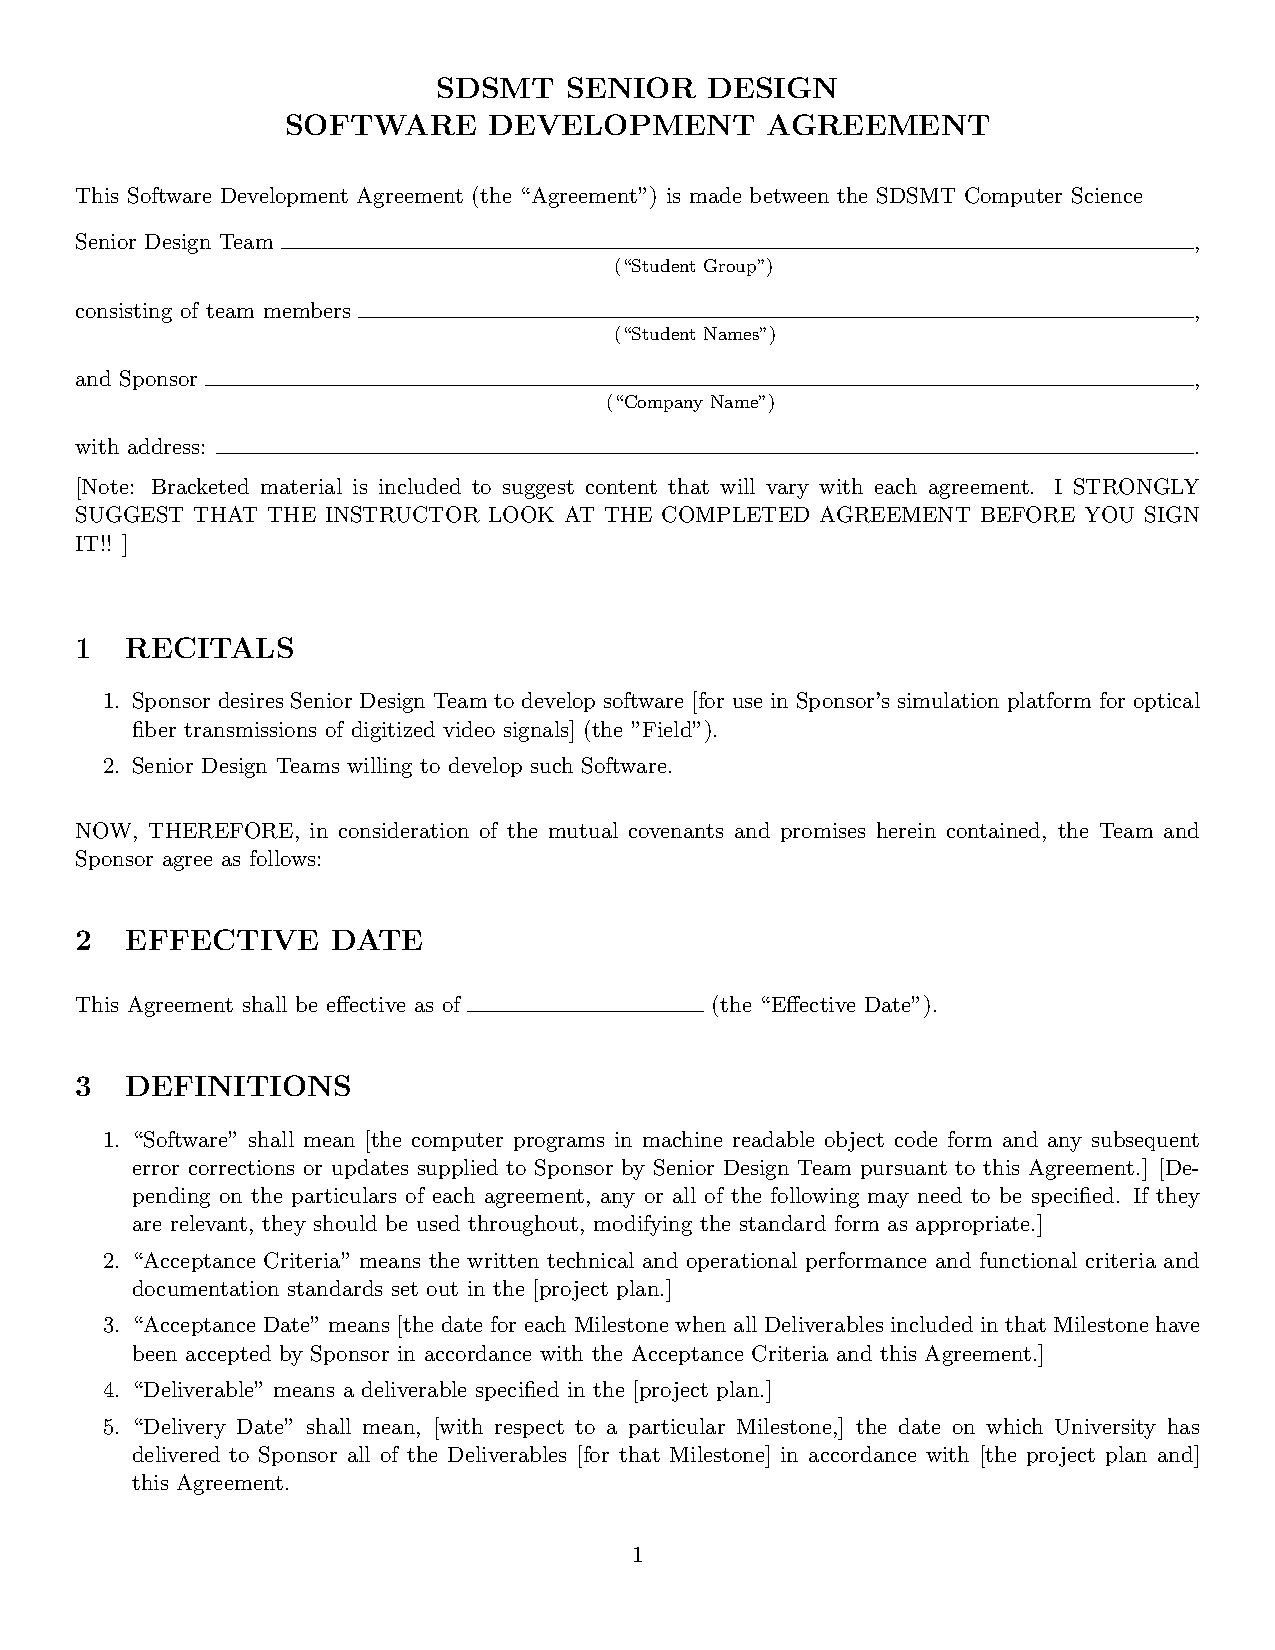
\includepdf[pages={1-5}]{InputDocs/SoftwareContract.pdf}

% In our style file, appendices are numbered with capital letters
\appendix

\chapter{Product Description}
% !TEX root = DesignDocument.tex

\section{Project Title} 
Crowd Science Mapper         

\section{Proposed/Advised by}   
Dr. Mengyu Qiao        
	
\section{Project Description}

Crowd Science (also known as Citizen Science) aims at soliciting ideas, findings, and information to support scientific research, which could reduce time and cost for data acquisition and enhance the accuracy and generality of research results.  Inspired by USGS Did You Feel It (DYFI) project, USGS Butterflies and Moths of North America (BAMONA) project, and Cornell’s eBird project, a group of professors and students from SDSMT partnered with SGT, Inc. to develop a Landscape Change Mapper (LC Mapper) system, which provides a mechanism for citizens and scientists to identify and track landscape change, thus extending the observational resources available to scientists and deepening the awareness and understanding of ecological issues by the public participants.

In recognition of the growing demand for crowd-sourcing in scientific research and the commonalities in various websites relying on citizens to assist in tracking and reporting science as it is happening, it will be helpful to develop a set of generic crowd-sourcing system framework and tool-kits, which can be customized by ordinary users with no programming experience using graphical user interface. The configurable features of the framework may include user input and display items, database design, digital map, web-page color and style, logo, etc. 

The Crowd Science Mapper will be a proof-of-concept project which spans across the areas of GIS/geospatial, cloud, crowd sourcing, citizen science, mobile applications, agile development, open source software, and open source data. The expected product comprises three components: 1) a configurable website that allows public participants to report and view events with visual help of a digital map; 2) a configurable mobile application with the same core features of the public website; 3) an administration website that allows administrators to customize and modify the public system design using graphical user interface, and allows scientists and moderators to control and analyse users’ reports.

\section{Useful Links}
USGS Did You Feel It website: http://earthquake.usgs.gov/earthquakes/dyfi
USGS Butterflies and Moths of North America website:  http://www.butterfliesandmoths.org
Cornell’s eBird website: http://ebird.org/content/ebird
SDSMT-SGT Landscape Change Mapper website: http://54.244.242.86/

\section{Project Duration}  Two semesters.

\section{Technical Areas Encompassed} 
Web development, Database, Mobile development

\section{Number of Students/Disciplines required} 4 Computer Science



%%\chapter{Publications}   %% Research track 
%%% !TEX root = DesignDocument.tex


Research Track:  
This chapter will include any publications generated from the research.  Most likely these will be preprints and one will just include the pdf.

%\includepdf[pages={1-5}]{Pub1.pdf}



\chapter{Sprint Reports}
% !TEX root = SystemTemplate.tex


\section{Sprint Report \#1}
% !TEX root = sprints_wrapper.tex

\subsection{Team Members}
Hannah Aker and Jiasong Yan
\subsection{Project Sponsors}
Dr. Mengyu Qiao and Gail Schmidt
\subsection{Sponsor/User Description}
\subsubsection{User Description}
Primary users will be the everyday citizen, interested in reporting some event, such as butterfly sighting, geological or landscape changes, etc. Secondary users will be academics and researchers who will use the gathered information in their research, they will be administrators of this data.
\subsubsection{Project Goal}
The goal of this project to improve on the idea originally presented in the Landscape Change Mapper, and expand on it to create a flexible interface for other kinds of events.
\subsubsection{User Needs}
Primary users need all the core fonctionality of the Landscape Change Mapper to be maintained.These functions include, but are not limited to:
\begin{itemize}
\item Visual map representation of events
\item Detailed event list
\item Event reporting interface
\item New user registration
\item User login
\end{itemize}
Users also need to be able to select which set of events they would like to view.
Administrators need to be able to customize a set of events to fit my needs. This may include user input and display items, database design, digital map, webpage color and style, logo, etc. Administrators will also need to be able to edit existing event reports.
\subsection{Project Overview}
The Crowd Science Mapper will be a generic crowdsourcing system framework and toolkits, which can be customized by ordinary users with no programming experience using graphical user interface
\subsection{Project Environment}
\subsubsection{Project Boundaries}
While the previous project included a mobile application, this project will not because the team is smaller. This project will be solely web-based. 
\subsubsection{Project Context}
This project will use the same general context that the Landscape Change Mapper used.  
\subsubsection{Technical Environment}
This project will use the same enviroment used in the Landscape Change Mapper. This will use HTML, PHP and Java Script to connect to a Mongo Database, and was hosted on an Apache 2.2 Server.
\subsubsection{Current systems overview}
The Landscape Change Mapper webpages used HTML, PHP and Java Script to connect to a Mongo Database, and was hosted on an Apache 2.2 Server. The webpage contained a map of events, detailed event list, event reporting interface, user login, and new user registration. The project included a mobile app with an event reporting interface. 
\subsection{Project Deliverables}
The project deliverable will be a proof-of-concept webpage with the features listed in the backlog.
\subsection{Backlog}
The following features need to be added to this project:
\begin{itemize}
\item Visual map representation of events
\item Detailed event list
\item Event reporting interface
\item New user registration
\item User login
\item User selection of data set to view
\item Administrator login
\item Administrator customization of event sets, including user input and display items, database design, digital map, webpage color and style, logo, etc. 
\item Administrator editing of existing event reports
\end{itemize}
\subsection{Potential Issues}
Potential issues might stem from using Java Script to interface with the Mongo DB. We don't have much prior experience with these specific tools, though we have used similar tools.


\section{Sprint Report \#2}

\section{Sprint Report \#3}

\section{Sprint Report ...}


\chapter{Industrial Experience and Resumes}
% !TEX root = ../SystemTemplate.tex
\section{ABET:  Industrial Experience Reports}

\subsection{Hannah Aker}

{\bf AFMC-OCALC, 76th SMXG, 555th MXDED}
SMART Intern
Summer 2014, Summer 2015
Oklahoma City, OK
\begin{itemize}
\item Designed and implemented software tool to view and edit aircraft engine data files for use in developing and testing CETADS (Comprehensive Engine Trending and Diagnostics System), using C\#, Windows Forms, WPF, XAML, and MVVM architecture. 
\item Summer 2014: created proof of concept program with complete functionality in Windows Forms, and created test cases for CETADS by hand using a hex editor. 
\item Summer 2015: improved original program using WPF, XAML, and MVVM structure, then recreated the program for a different engine.
\item Supervisor: Francesco Whittenberger, francesco.whittenberger@us.af.mil
\end{itemize}

\section{Resumes}

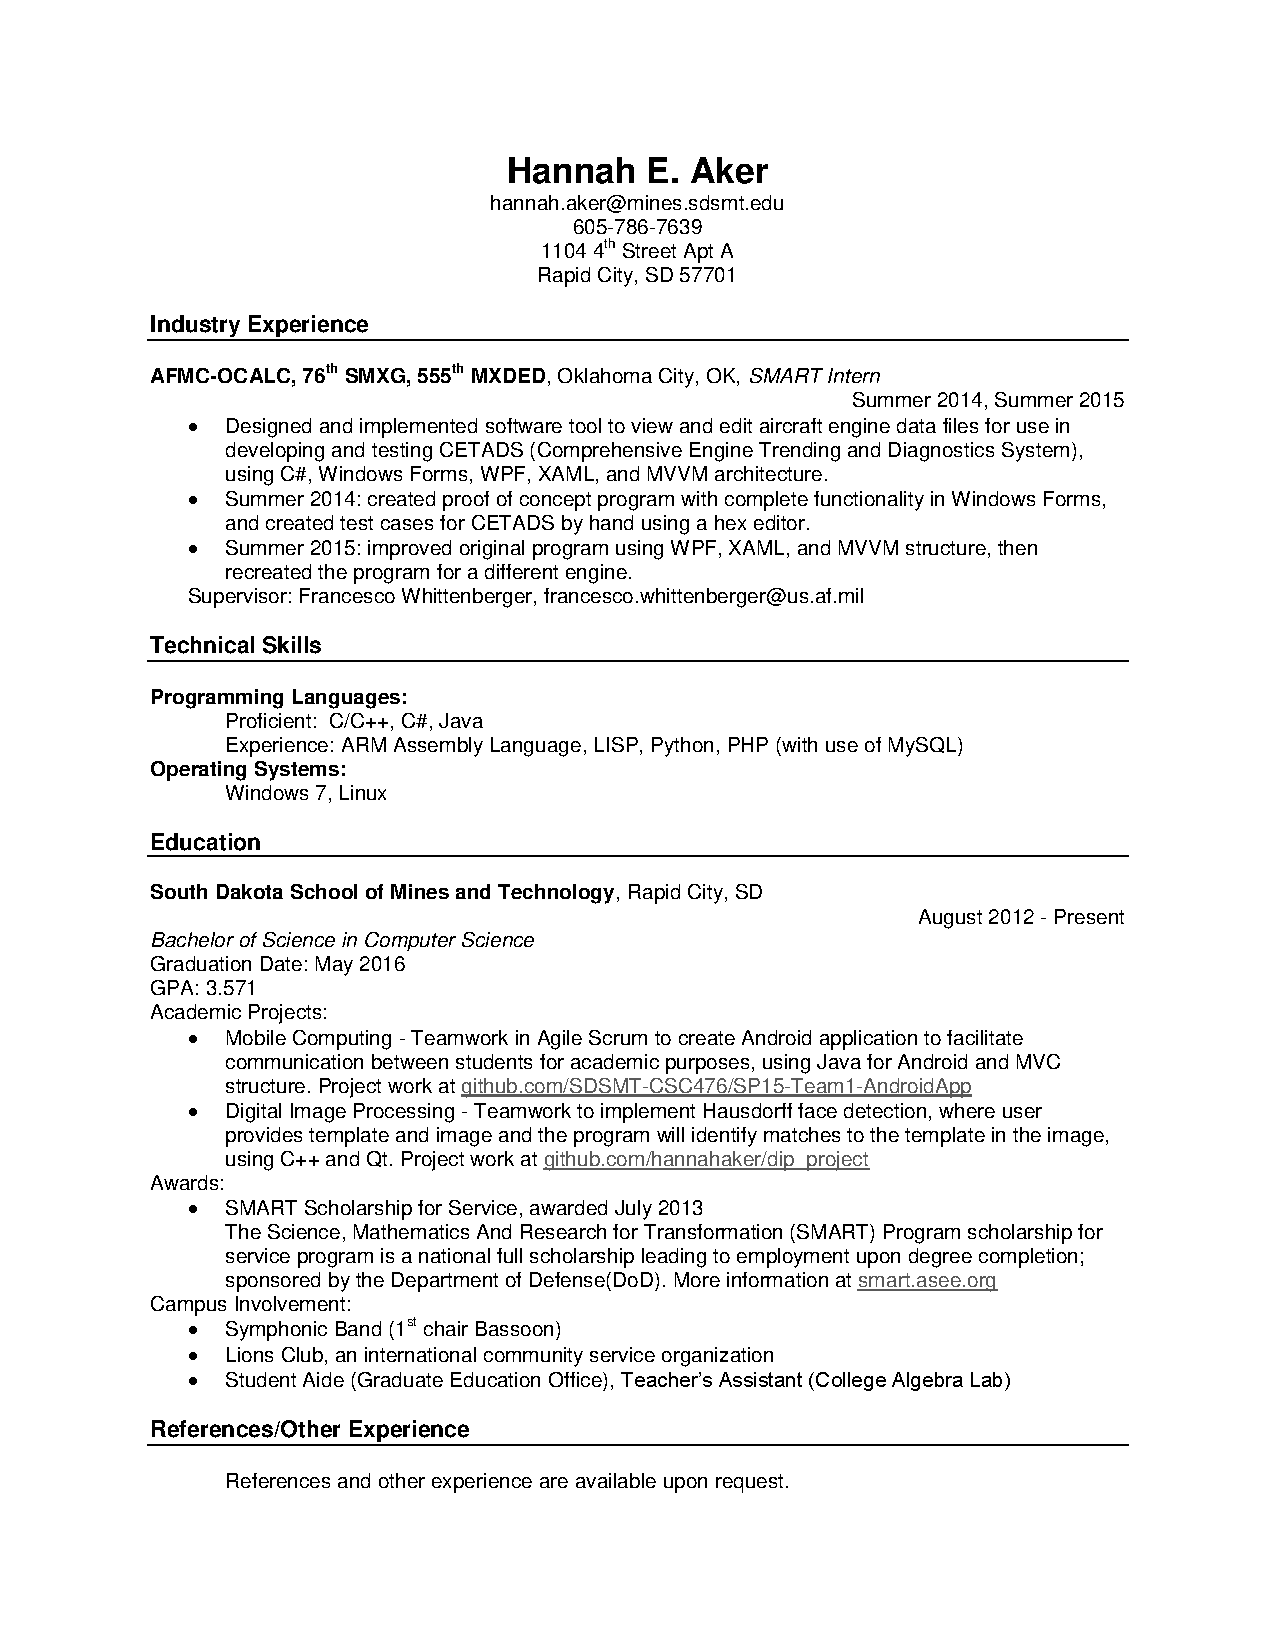
\includepdf[pages={1-2}]{./InputDocs/AkerResume9-8-2015.pdf}

%    \includepdf[pages={1}]{report.pdf}  %% example of limited page include

%     \includepdf{resume1.pdf}
%     \includepdf{resume2.pdf}
%     \includepdf{resume3.pdf}









\chapter{Acknowledgment}
\label{SpecialThanks}  
Thanks  

\chapter{Supporting Materials}
% !TEX root = ../SystemTemplate.tex

\section{Live Prototype}
Live prototype can be found at: \url{http://52.23.113.55}

\section{Screenshots}
Figure~\ref{prototype_main}. is a screenshot of the Crowd Science Mapper main page, as of the end of Sprint 3.  Figure~\ref{prototype_login}. is a screenshot of the Crowd Science Mapper login page, as of the end of Sprint 3. Figure~\ref{prototype_register}. is a screenshot of the Crowd Science Mapper register page, as of the end of Sprint 3.

\begin{figure}[tbh]
\begin{center}
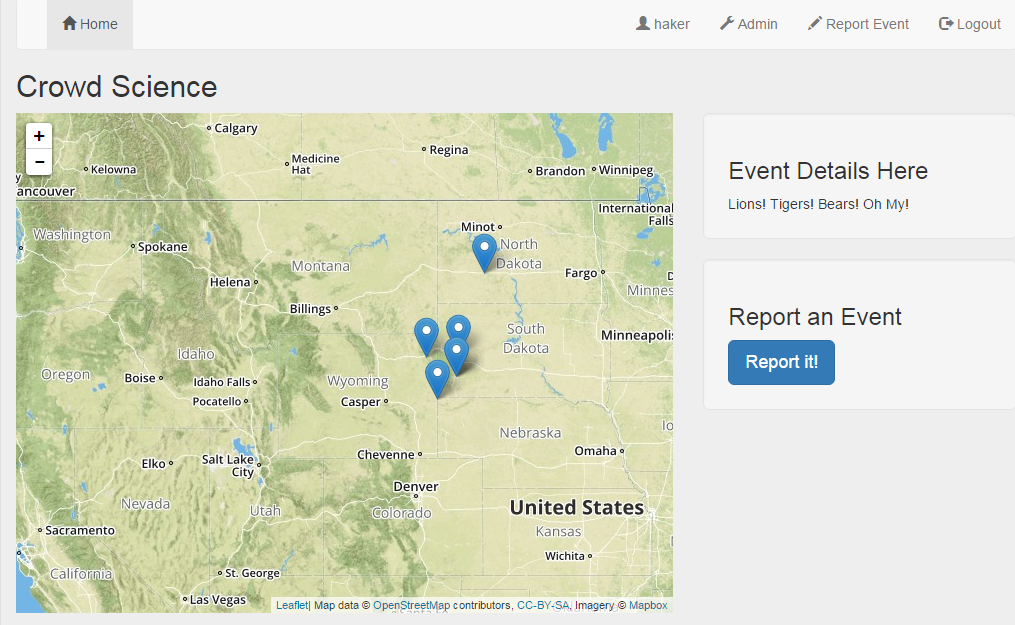
\includegraphics[width=0.75\textwidth]{./Images/prototype_main.png}
\end{center}
\caption{Screenshot of Crowd Science Main Page\label{prototype_main}}
\end{figure}

\begin{figure}[tbh]
\begin{center}
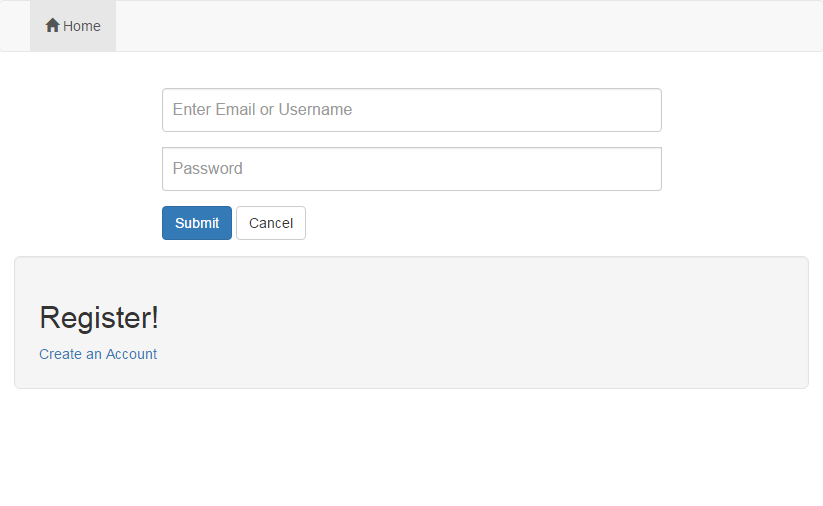
\includegraphics[width=0.75\textwidth]{./Images/prototype_login.png}
\end{center}
\caption{Screenshot of Crowd Science Main Page\label{prototype_login}}
\end{figure}

\begin{figure}[tbh]
\begin{center}
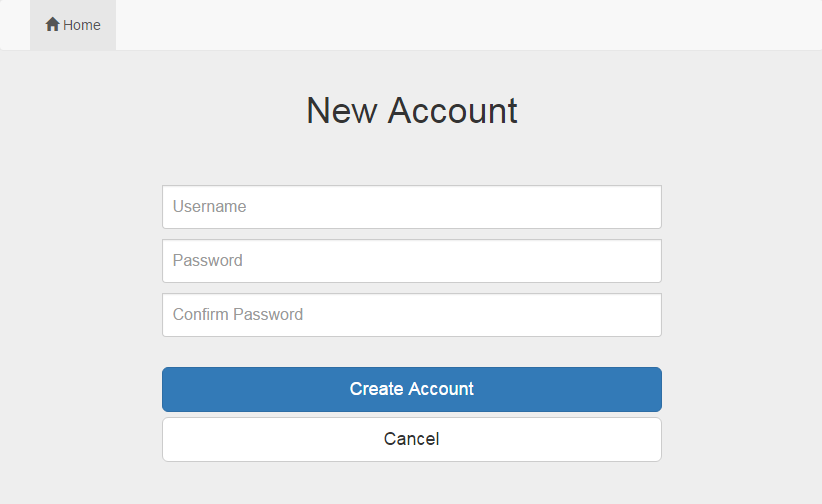
\includegraphics[width=0.75\textwidth]{./Images/prototype_register.png}
\end{center}
\caption{Screenshot of Crowd Science Main Page\label{prototype_register}}
\end{figure}

% chapters in backmatter don't have numbers, but they appear in the
% table of contents, and are numbered BM-X where X is the page number
% relative to where the backmatter begins.
\backmatter

%% Example
%\chapter{Course Syllabus}
%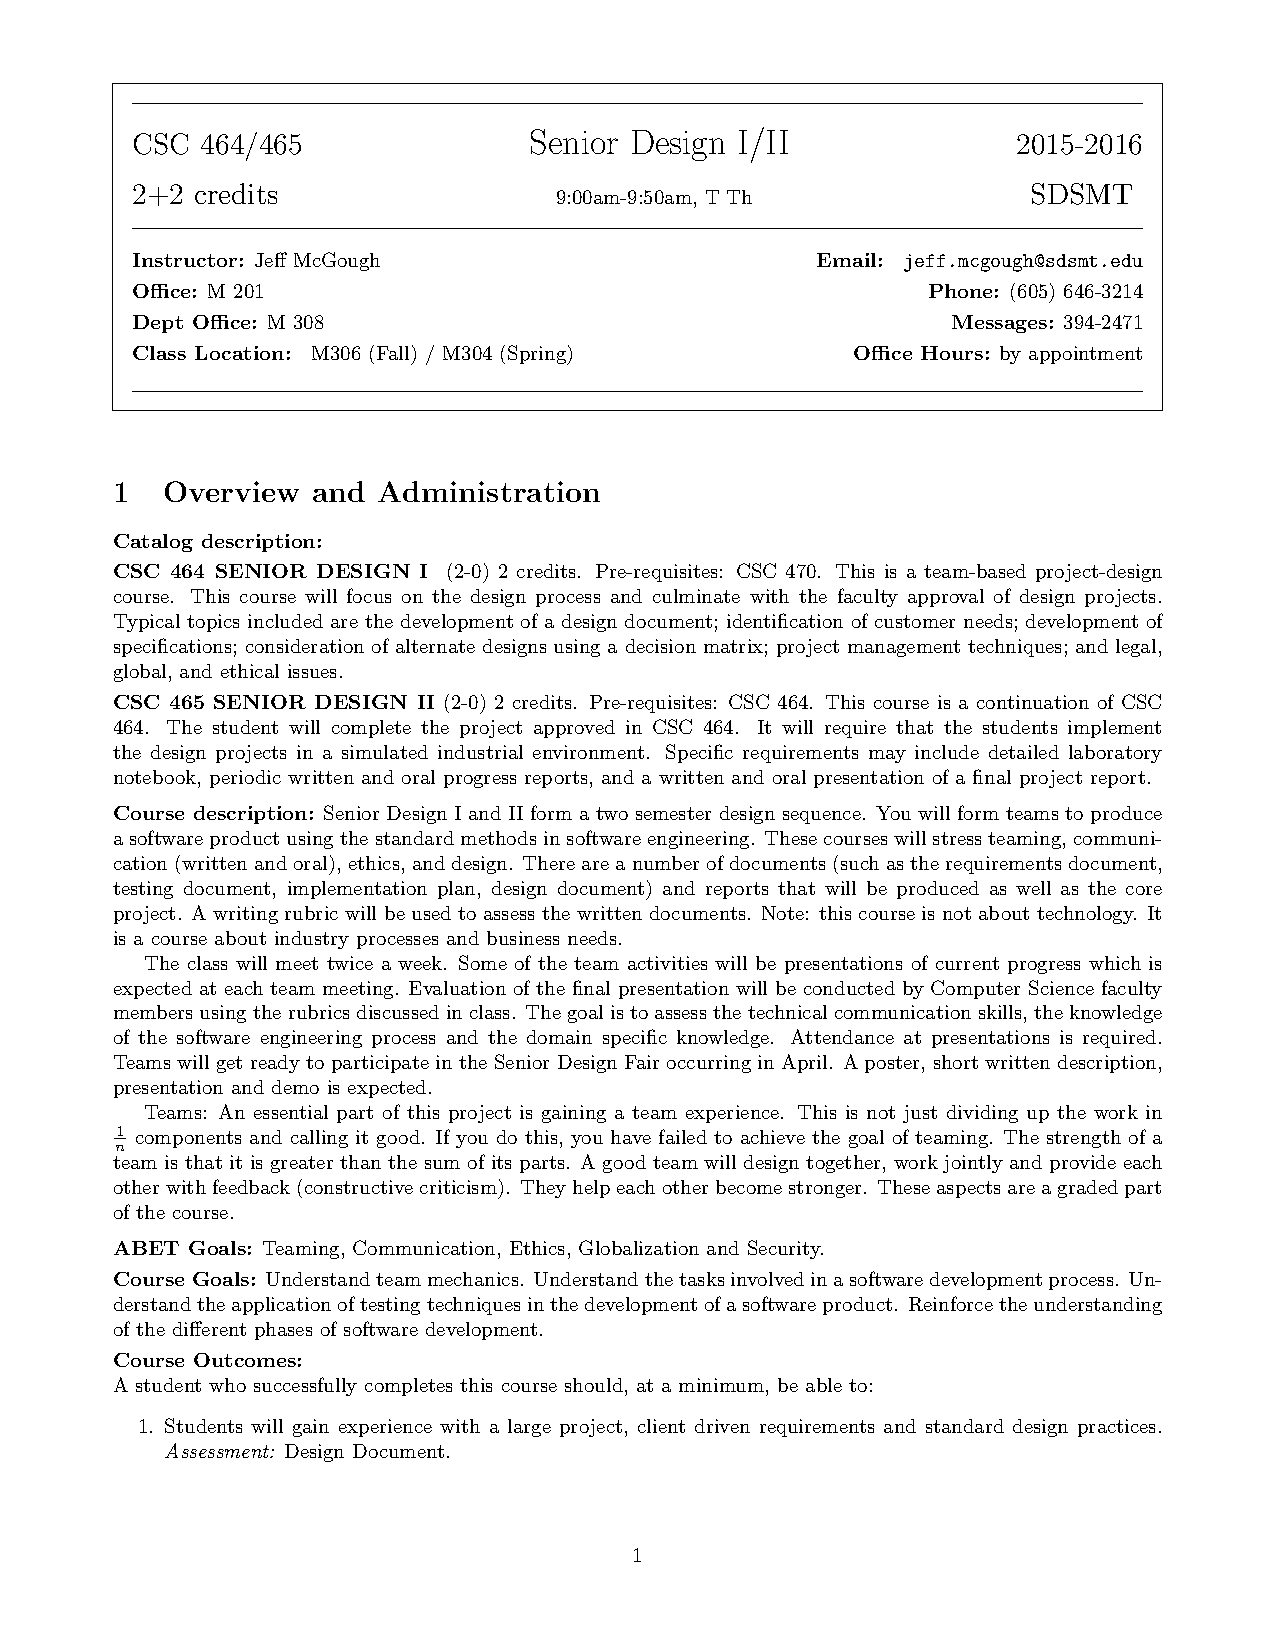
\includepdf[pages={1-17}]{syllabus.pdf}

%%% Remove after reading
%%\chapter{\LaTeX\ Example}
%%% !TEX root = DesignDocument.tex


\LaTeX\xspace sample file:  {\color{red} Remove from submitted materials}

\section{Introduction}
This is a sample input file.  Comparing it with the output it
generates can show you how to produce a simple document of
your own.

\section{Ordinary Text}  % Produces section heading.  Lower-level
                                    % sections are begun with similar 
                                    % \subsection and \subsubsection commands.

The ends  of words and sentences are marked 
  by   spaces. It  doesn't matter how many 
spaces    you type; one is as good as 100.  The
end of   a line counts as a space.

One   or more   blank lines denote the  end 
of  a paragraph.  

Since any number of consecutive spaces are treated like a single
one, the formatting of the input file makes no difference to
      \TeX,         % The \TeX command generates the TeX logo.
but it makes a difference to you.  
When you use
      \LaTeX,       % The \LaTeX command generates the LaTeX logo.
making your input file as easy to read as possible
will be a great help as you write your document and when you
change it.  This sample file shows how you can add comments to
your own input file.

Because printing is different from typewriting, there are a 
number of things that you have to do differently when preparing 
an input file than if you were just typing the document directly.  
Quotation marks like 
       ``this'' 
have to be handled specially, as do quotes within quotes: 
       ``\,`this'                  % \, separates the double and single quote.
        is what I just 
        wrote, not  `that'\,''.  

Dashes come in three sizes: an 
       intra-word 
dash, a medium dash for number ranges like 
       1--2, 
and a punctuation 
       dash---like 
this.

A sentence-ending space should be larger than the space between words
within a sentence.  You sometimes have to type special commands in
conjunction with punctuation characters to get this right, as in the
following sentence.
       Gnats, gnus, etc.\    % `\ ' makes an inter-word space.
       all begin with G\@.   % \@ marks end-of-sentence punctuation.
You should check the spaces after periods when reading your output to
make sure you haven't forgotten any special cases.
Generating an ellipsis 
       \ldots\    % `\ ' needed because TeX ignores spaces after 
                  % command names like \ldots made from \ + letters.
                  %
                  % Note how a `%' character causes TeX to ignore the 
                  % end of the input line, so these blank lines do not
                  % start a new paragraph.
with the right spacing around the periods 
requires a special  command.  

\TeX\ interprets some common characters as commands, so you must type
special commands to generate them.  These characters include the
following: 
       \$ \& \% \# \{ and \}.

In printing, text is emphasized by using an
       {\em italic\/}  % The \/ command produces the tiny extra space that
                       % should be added between a slanted and a following
                       % unslanted letter.
type style.  

\begin{em}
   A long segment of text can also be emphasized in this way.  Text within
   such a segment given additional emphasis 
          with\/ {\em Roman} 
   type.  Italic type loses its ability to emphasize and become simply
   distracting when used excessively.  
\end{em}

It is sometimes necessary to prevent \TeX\ from breaking a line where
it might otherwise do so.  This may be at a space, as between the
``Mr.'' and ``Jones'' in
       ``Mr.~Jones'',        % ~ produces an unbreakable interword space.
or within a word---especially when the word is a symbol like
       \mbox{\em itemnum\/} 
that makes little sense when hyphenated across 
       lines.

Footnotes\footnote{This is an example of a footnote.}
pose no problem.

\TeX\ is good at typesetting mathematical formulas like
       \( x-3y = 7 \) 
or
       \( a_{1} > x^{2n} / y^{2n} > x' \).
Remember that a letter like
       $x$        % $ ... $  and  \( ... \)  are equivalent
is a formula when it denotes a mathematical symbol, and should
be treated as one.

\section{Displayed Text}

Text is displayed by indenting it from the left margin.
Quotations are commonly displayed.  There are short quotations
\begin{quote}
   This is a short a quotation.  It consists of a 
   single paragraph of text.  There is no paragraph
   indentation.
\end{quote}
and longer ones.
\begin{quotation}
   This is a longer quotation.  It consists of two paragraphs
   of text.  The beginning of each paragraph is indicated
   by an extra indentation.

   This is the second paragraph of the quotation.  It is just
   as dull as the first paragraph.
\end{quotation}
Another frequently-displayed structure is a list.
The following is an example of an {\em itemized} list.
\begin{itemize}
   \item  This is the first item of an itemized list.  Each item 
          in the list is marked with a ``tick''.  The document
          style determines what kind of tick mark is used.

   \item  This is the second item of the list.  It contains another
          list nested inside it.  The inner list is an {\em enumerated}
          list.
          \begin{enumerate}
              \item This is the first item of an enumerated list that
                    is nested within the itemized list.

              \item This is the second item of the inner list.  \LaTeX\
                    allows you to nest lists deeper than you really should.
          \end{enumerate}
          This is the rest of the second item of the outer list.  It
          is no more interesting than any other part of the item.
   \item  This is the third item of the list.
\end{itemize}
You can even display poetry.
\begin{verse}
   There is an environment for verse \\    % The \\ command separates lines
   Whose features some poets will curse.   % within a stanza.

                           % One or more blank lines separate stanzas.

   For instead of making\\
   Them do {\em all\/} line breaking, \\
   It allows them to put too many words on a line when they'd 
   rather be forced to be terse.
\end{verse}

Mathematical formulas may also be displayed.  A displayed formula is
one-line long; multi-line formulas require special formatting
instructions.
   \[  x' + y^{2} = z_{i}^{2}\]
Don't start a paragraph with a displayed equation, nor make
one a paragraph by itself.

\section{Build process}

To build \LaTeX\ documents you need the latex program.  It is free and available on all operating systems.   Download and install.  Many of us use the TexLive distribution and are very happy with it.    You can use a editor and command line or use an IDE.  To build this document via command line:

\begin{verbatim}
alta>  pdflatex SystemTemplate
\end{verbatim}
If you change the bib entries, then you need to update the bib files:
\begin{verbatim}
alta>  pdflatex SystemTemplate
alta>  bibtex SystemTemplate
alta>  pdflatex SystemTemplate
alta>  pdflatex SystemTemplate
\end{verbatim}

The template files provided also contain a Makefile, which will
make things much easier.  

\section*{Acknowledgment}
Thanks to Leslie Lamport.  






\end{document}
